\chapter{概要设计}

% 本章主要阐述了系统架构、系统各模块具体架构和数据库概要设计等方面的内容,通过借助系统结构图和活动图来描述各功能实现的基本原理,为第五章的详细设计奠定了基础。

本章重点介绍了系统结构、数据库系统各单元的结构以及系统概要结构等方面的内容,通过利用系统结构图与过程图来说明各功能实现的基本原理,为第五章的详细分析打下了基础。
\section{系统架构设计}

% 系统的功能模块按照微服务的拆分原则拆分成了四个部分,主要为存储管理模块、权限控制模块、认证中心模块和API网关模块。系统整体的逻辑架构如图\ref{fig:系统逻辑架构图}所示。
系统的功能模组根据微服务的拆分原理分拆为了四大模块,主要分为存储管理功能、客户信息管理功能、应用服务功能,以及API的网关功能。
\begin{figure}[h]
    \centering
    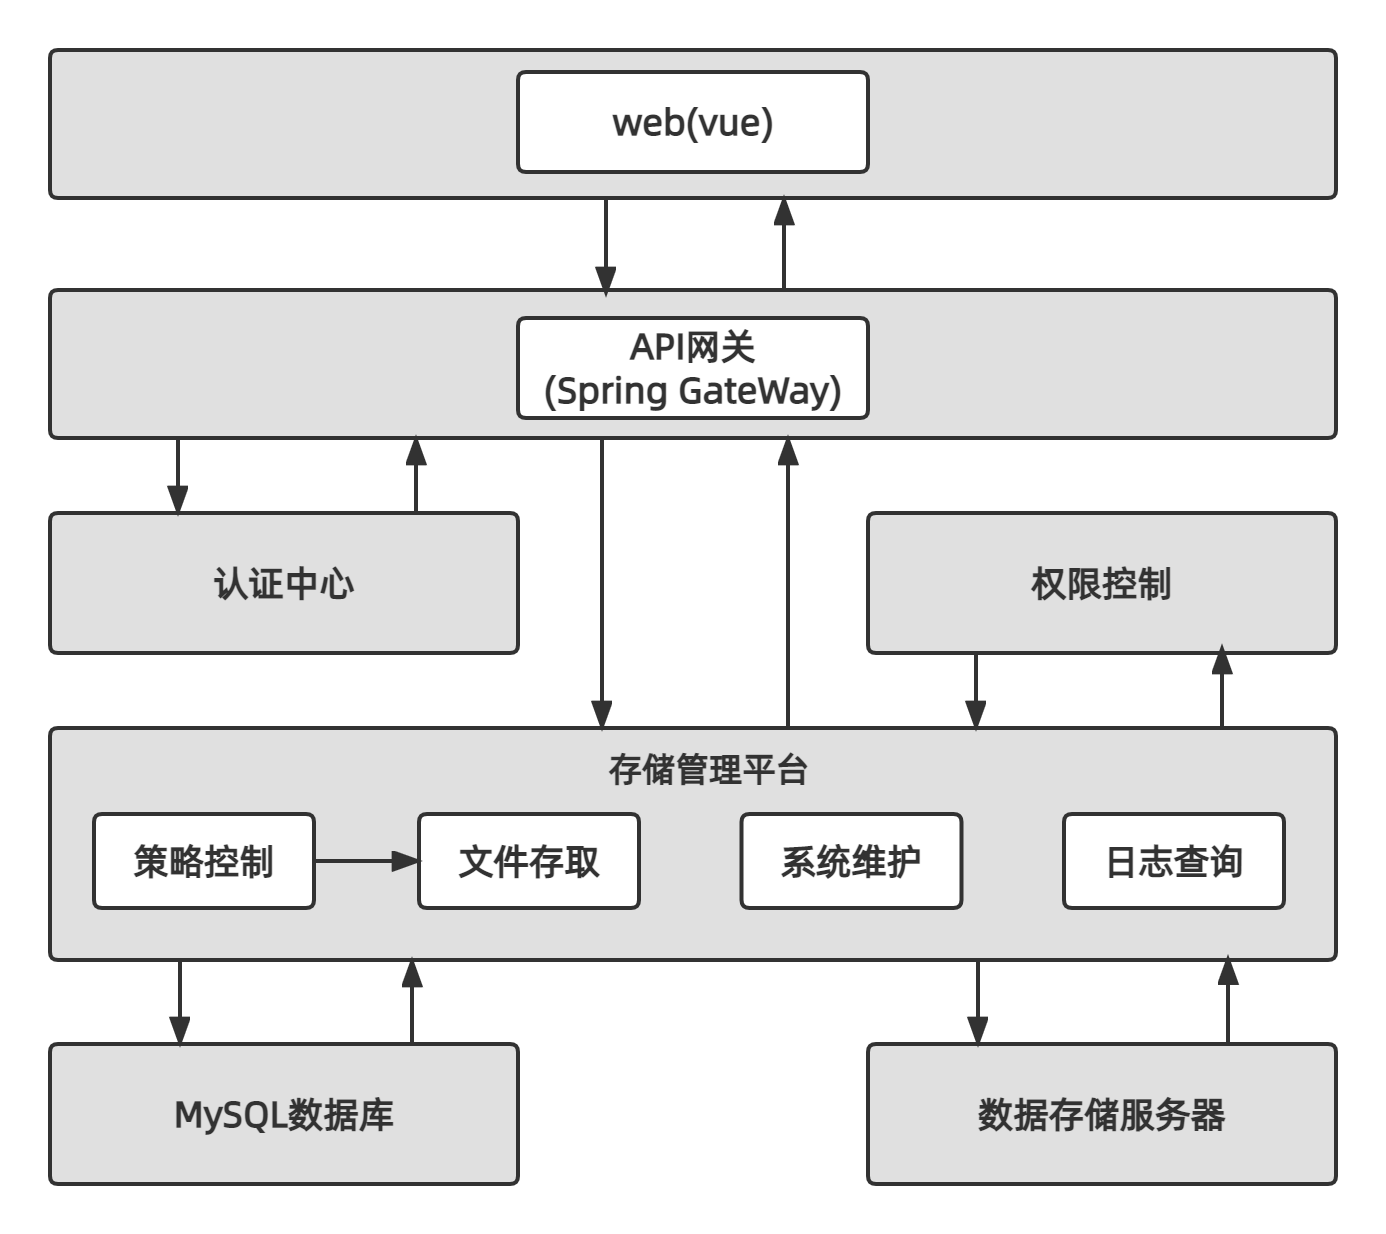
\includegraphics[width=1\textwidth]{my_figures/chapter4/系统逻辑架构.png}
    \caption{系统逻辑架构图}
    \label{fig:系统逻辑架构图}
%     \note{注:图注的内容不宜放到图题中。}
\end{figure}

% 其中,API网关主要负责接收从前端发过来的请求,并使用HTTP协议与其他三个微服务进行交互,网关微服务的端口是整个系统对外暴露的唯一端口。认证中心模块主要负责对用户的身份进行
% 校验。权限控制模块主要负责对用户的账号、角色和权限等信息进行管理。存储管理平台是整个系统的核心业务模块,同时与MySQL数据库和数据存储服务器相连,MySQL数据库主要存储管理
% 平台上用户的账号、角色和权限等相关信息,数据存储服务器是用户上传或下载文件的位置,是整个系统最关键的部分。

% 其中,API网关服务主要功能是接受来自前端发过来的请求,并通过HTTP协议和另外三个微服实现通讯,而网关微服的接口则是整个服务
% 对外暴露的惟一接口。认证中心模块,主要承担对认证客户的责任身份进行校验。用户管理模块主要承担对客户的账号、角色和授权等
% 信息进行了管理。

存储管理平台是整个管理系统的核心服务模块,同时也与MySQL数据库和数据存放服务器相连接,MySQL数据库中主要
存储管理平台上使用者的帐号、角色和权限等有关信息,数据存储服务器是用户上传或下载文件的位置,是整个系统
最关键的部分。

\section{系统功能模块架构}

\begin{figure}[h]
    \centering
    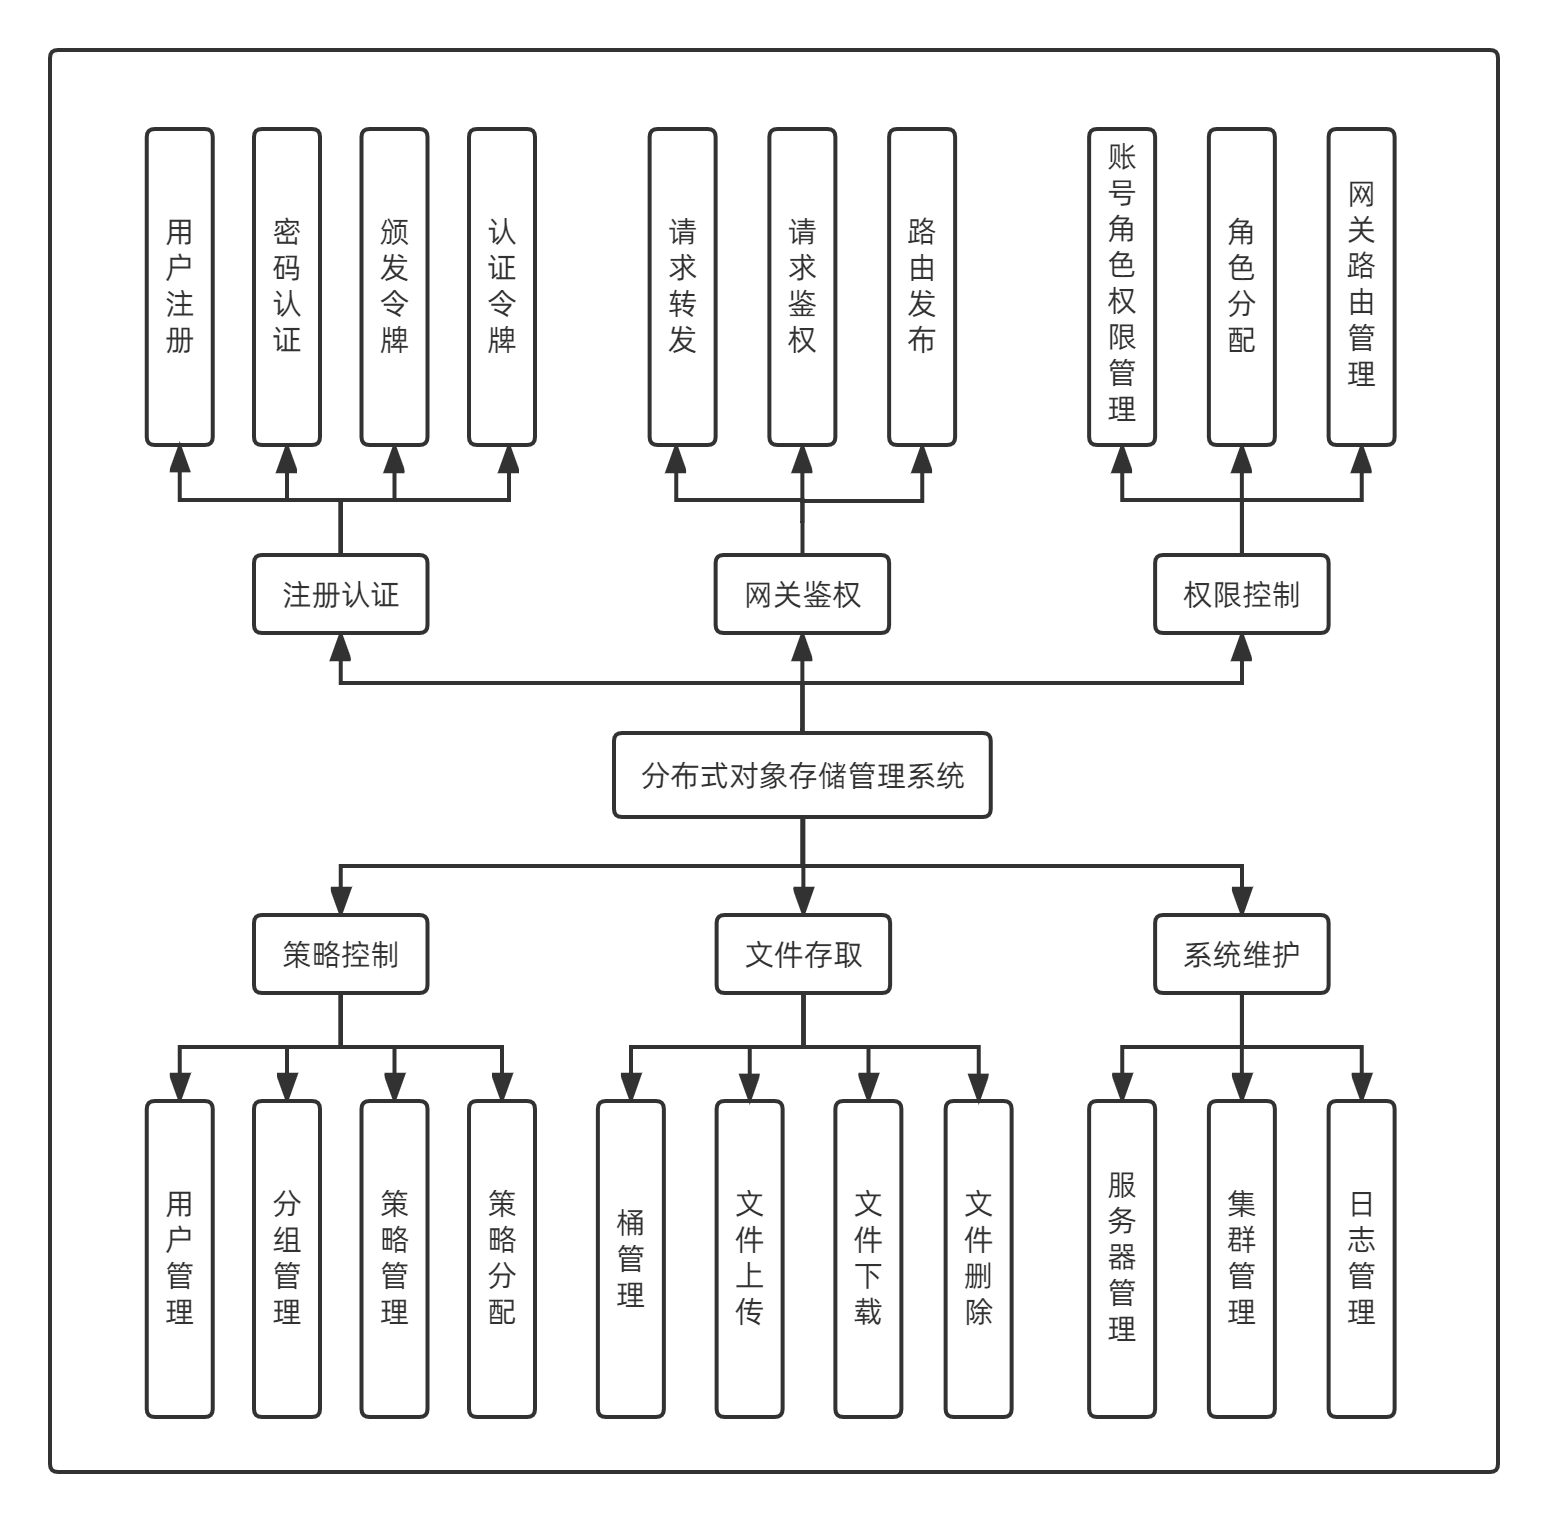
\includegraphics[width=1\textwidth]{my_figures/chapter4/系统功能模块.png}
    \caption{系统功能模块}
    \label{fig:系统功能模块}
%     \note{注:图注的内容不宜放到图题中。}
\end{figure}


% 根据软件工程中软件项目高内聚、 低耦合的特点, 将分布式对象存储管理系统按功能划分为认证模块、网关鉴权模块、权限控制模块、策略控制模块、文件存取模块和系统维护模块等六个模
% 块。每个模块又可以划分为各个功能小模块,注册认证模块包含用户注册子模块、 用户名密码认证子模块、 颁发令牌子模块和认证令牌子模块,网关鉴权模块包含请求转发子模块、请求鉴权子模
% 块和路由发布子模块,权限控制模块包含账号角色权限管理子模块、角色分配子模块和网关路由管理子模块,策略控制模块包含用户管理子模块、分组管理子模块、策略管理子模块和策略分配
% 子模块,文件存取模块包含桶管理子模块、文件上传子模块、文件下载子模块和文件删除子模块,系统维护模块包含服务器管理子模块、集群管理子模块和日志管理子模块。系统功能模块图如
% 图\ref{fig:系统功能模块}所示。

% 系统功能模块图与系统用例表\ref{系统用例表}并不是完全对应的, 系统用例表主要是根据用户的实际需求抽象出系统用例,而系统功能的模块图主要是根据系统功能的底层实现,将系统
% 划分为若干模块,这些模块继续划分为若干子模块。以文件存取模块为例,用户想进入文件存取模块首先必须登录管理系统,对于登录过程,为了实现系统的可拓展性,系统底层
% 将用户登录这个过程实际上经过了一系列的子过程,这些子过程分别访问了网关鉴权模块、注册认证模块和文件存取模块这三个模块,但用户并没有感觉到这些子过程的发生,这些访问
% 过程对于用户来说是透明的。一般情况下,系统用例表中的每一个用例都需要一个模块或多个模块共同配合才能实现。本文第四章和第五章主要根据系统实现细节,结合系统功能模块图\ref{fig:系统功能模块}
% 阐述系统的概要设计和详细设计,第三章和第六章主要根据用户的实际需求,结合系统用例表\ref{系统用例表}进行系统用例设计和测试。

针对软件工程中软件的高度内聚、低相互耦合的特性,将分布式数据存储管理技术按特性分类为认证系统、网关鉴权系统、权限管控系
统、策略控制模块、文件存取模块和系统维护模块等六个模块。这些功能都可区分成不同功能的子模块,用户管理功能包括用户角色授权控制子模块、角色配置子模块和网关路由控制子模块,策略管理功能包括用户管理子模块、分
组控制子模块、策略管理子模块和策略配置子模块,文档存储功能包括桶管理子模块、文档提交子模块、文档加载子模块和文档删除子
模块,系统维护功能包括服务器管理子模块、集群管理子模块和日志管理子模块。系统的功能模块示意图,如图四点二中所示。

系统的功能模块图和系统使用范围图三点二中并没有截然相对的,系统使用范围图主要是针对客户的具体要求抽象的统一用例,而系统
功能的单元图主要是针对系统功能的底层应用,把整个系统功能分割成若干个模块,而这些功能又可以细分为若干个子功能。以文件存
取模块为例,系统要进入文件存取模块首先需要经过注册管理系统,而对于注册过程来说,为实现管理系统的可扩展性,在管理系统底层
将用户注册的步骤中也经过了大量的子流程,而这些子流程中依次使用了网关鉴权功能、注册认证功能以及文件存取模块这三种功能,
但用户并没有感觉到这些子过程的发生,这些访问过程对于用户来说是透明的。通常情况下,在系统用例表中的每一条用例,都必须一个
模块或几个模块的共同配合,方可完成。本文第四章和第五章主要针对系统的实现细节,结合系统职能模型图四点二阐述系统的功能概
要设计和细节设计,而第三章和第六章则主要针对应用的现实需要,结合系统应用案例表三点二进行系统的应用案例设计与测试。

\section{系统各功能模块设计}

\subsection{注册认证模块}

% 本系统采用的是微服务架构,一个微服务可能部署多个实例,如果和传统的单体项目一样采用session/cookie 的方式来进行会话管理的话,这样必须保证用户的每次请求都到达
% 同一个实例上,同时随着用户量的增加,服务端需要耗费大量的内存空间来保存session,造成服务器内存紧张,而且从安全的角度,cookie很容易遭到拦截和盗用,存在一定的
% 安全隐患。

% 在微服务的架构下,常用的认证模式是基于token的认证模式。虽然有很多种不同的方式来实现基于token的身份验证,但业界广泛采用的实现方案是JSON Web Tokens(JWT) ,
% 事实上,JWT已经成为了业内标准。 基于token的认证方式是无状态的。为了判断用户的身份,服务器需要通过额外的计算来解析token的内容,这样做服务器可以节约空间,因为
% 不再需要花费额外的空间去记录已登录用户的信息,也不用在多实例部署时反复验证用户身份。

% 注册认证模块主要包含四个子模块,分别是用户注册子模块、用户名密码认证子模块、颁发令牌子模块和认证令牌子模块。注册认证模块的功能结构图如图
% \ref{fig:注册认证模块功能结构图}所示。

该服务使用的是微服务架构,每一个微型服务都可以配置成几个实例,但是如果与一般的小单体服务相比使用了session/cookie的形式
来实现会话控制功能的话,这样就必须确保客户的每个请求都在一个实例中,同时由于使用量的增加,服务器也必须消耗巨大的内部空间
来保护session,从而导致了服务器数据库内存紧缺,同时从安全性的考虑,cookie也极易受到截获和窃取,存在一定的安全隐患。

在微服务的标准框架里,最常见的认证方式就是采用 token 的认证方式。尽管有很多种不同的方法可以实现采用 token 的身份验证,
但目前业界最普遍使用的实现方法还是JSONWeb token s(JWT),而实际上,JWT早已形成了一个业界规范。由于token的验证方法是
无问题的。为确定客户的身分,系统必须使用额外的时间来分析token的信息,这样的系统能够节省存储空间,因此不再需要耗费额外
的空间去查询新注册客户的数据,而无须在多实例部署中重复校验客户身份。

% 用户验证系统主要包括四个种子模块,分别为用户注册子模块、用户名口令验证子模块、颁发令牌子模块和认证令牌子模块。注册认证
% 模块的功能结构图如图
% 4.3所示。

\begin{figure}[h]
    \centering
    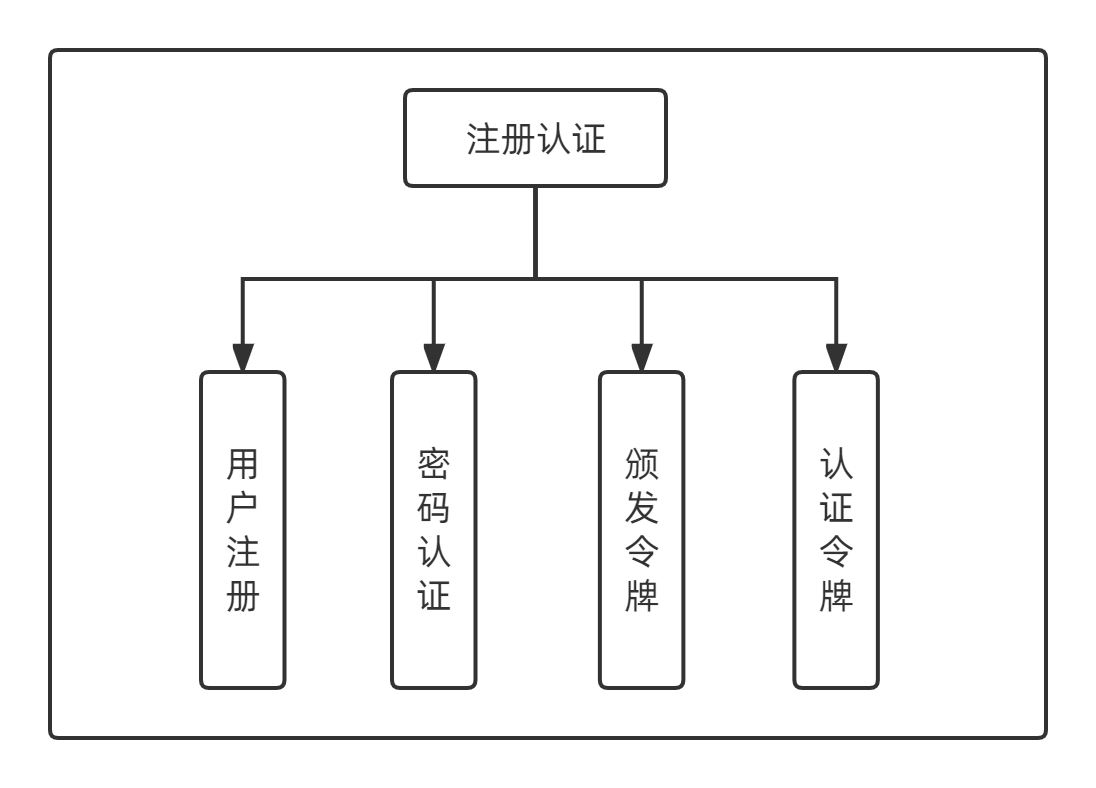
\includegraphics[width=0.8\textwidth]{my_figures/chapter4/注册认证模块功能结构图.png}
    \caption{注册认证模块功能结构图}
    \label{fig:注册认证模块功能结构图}
%     \note{注:图注的内容不宜放到图题中。}
\end{figure}

(1) 用户注册

% 该系统的注册用户主要有两种,一类是普通管理员,另一类是普通用户。普通管理员由于身份特殊,会有一定的限制。为了防止外部人员获得非法管理权限,超级管理员与公司内部
% 人员协商出了注册密钥。如果用户注册的是普通管理员,用户在注册账号时需要选择普通管理员的角色,并正确的填写对应的密钥,之后填写用户名、密码、校验码等常规信息。前
% 端首先会校验用户名和密码的格式,用户点击注册后,后端会判断用户填写的密钥和对应的角色密钥是否匹配,如果不匹配则直接向前端返回错误信息。如果用户注册的是普通用户,
% 用户在注册账号时不需要进行密钥比对,可直接注册,只要保证用户名和密码格式正确即可。当然,无论是注册哪种角色的用户,都要求是全英文的用户名,而且首先会检查用户名是否存在,若用户名已存在,则会
% 向前端报错,要求重新输入正确的用户名。在经过校验后,管理员用户或普通用户都会根据用户名生成相应的AccessKey和SecretKey,在远程存储服务器上创建对应的管
% 理员用户和普通用户,且会为普通用户分配相应的存储空间。然后,系统会将用户输入的账号信息插入数据库的用户表中,将返回的主键 ID 和角色 ID 作
% 为一条记录再插入到用户角色关联表中。最后会给超级管理员和注册用户发送用户创建邮件通知,提示用户创建成功。用户注册活动图如图\ref{fig:用户注册活动图}所示。

本系统的登录客户大致分为二种,第一类是正常客户,另一类则是正常客户。普通管理员由于身份特殊,会有一定的限制。为避免外部员
工获得非法管理权限,超级管理员和企业内部人员之间协商出了注册密钥。如果用户所注册的是普通管理员,用户在登录账号时就必须
选择普通管理员的角色,并准确的选择了相应的密钥,如果用户注册的是普通用户,用户在注册账号时不需要进行密钥比对,可直接注册,只要保证用户名和密码格式正确即可。当然,无论是注册哪种
角色的用户,都要求是全英文的用户名,而且首先会检查用户名是否存在,若用户名已存在,则会向前端报错,要求重新输入正确的用户
名。在经过校验后,管理员用户或普通用户都会根据用户名生成相应的AccessKey和 SecretKey,在远程存储服务器上创建对应的管理
员用户和普通用户,且会为普通用户分配相应的存储空间。之后,系统就会把所有用户输入的帐号信息进入数据库的用户列表中,将返回
的主键ID与角色ID成为同一个记录,再插入到所有用户角色关联列表中。最后,会向超级管理员和已注册用户发送用户创建的邮件通知,
提示用户创建成功。用户注册活动图如图4.4所示。

\begin{figure}[h]
    \centering
    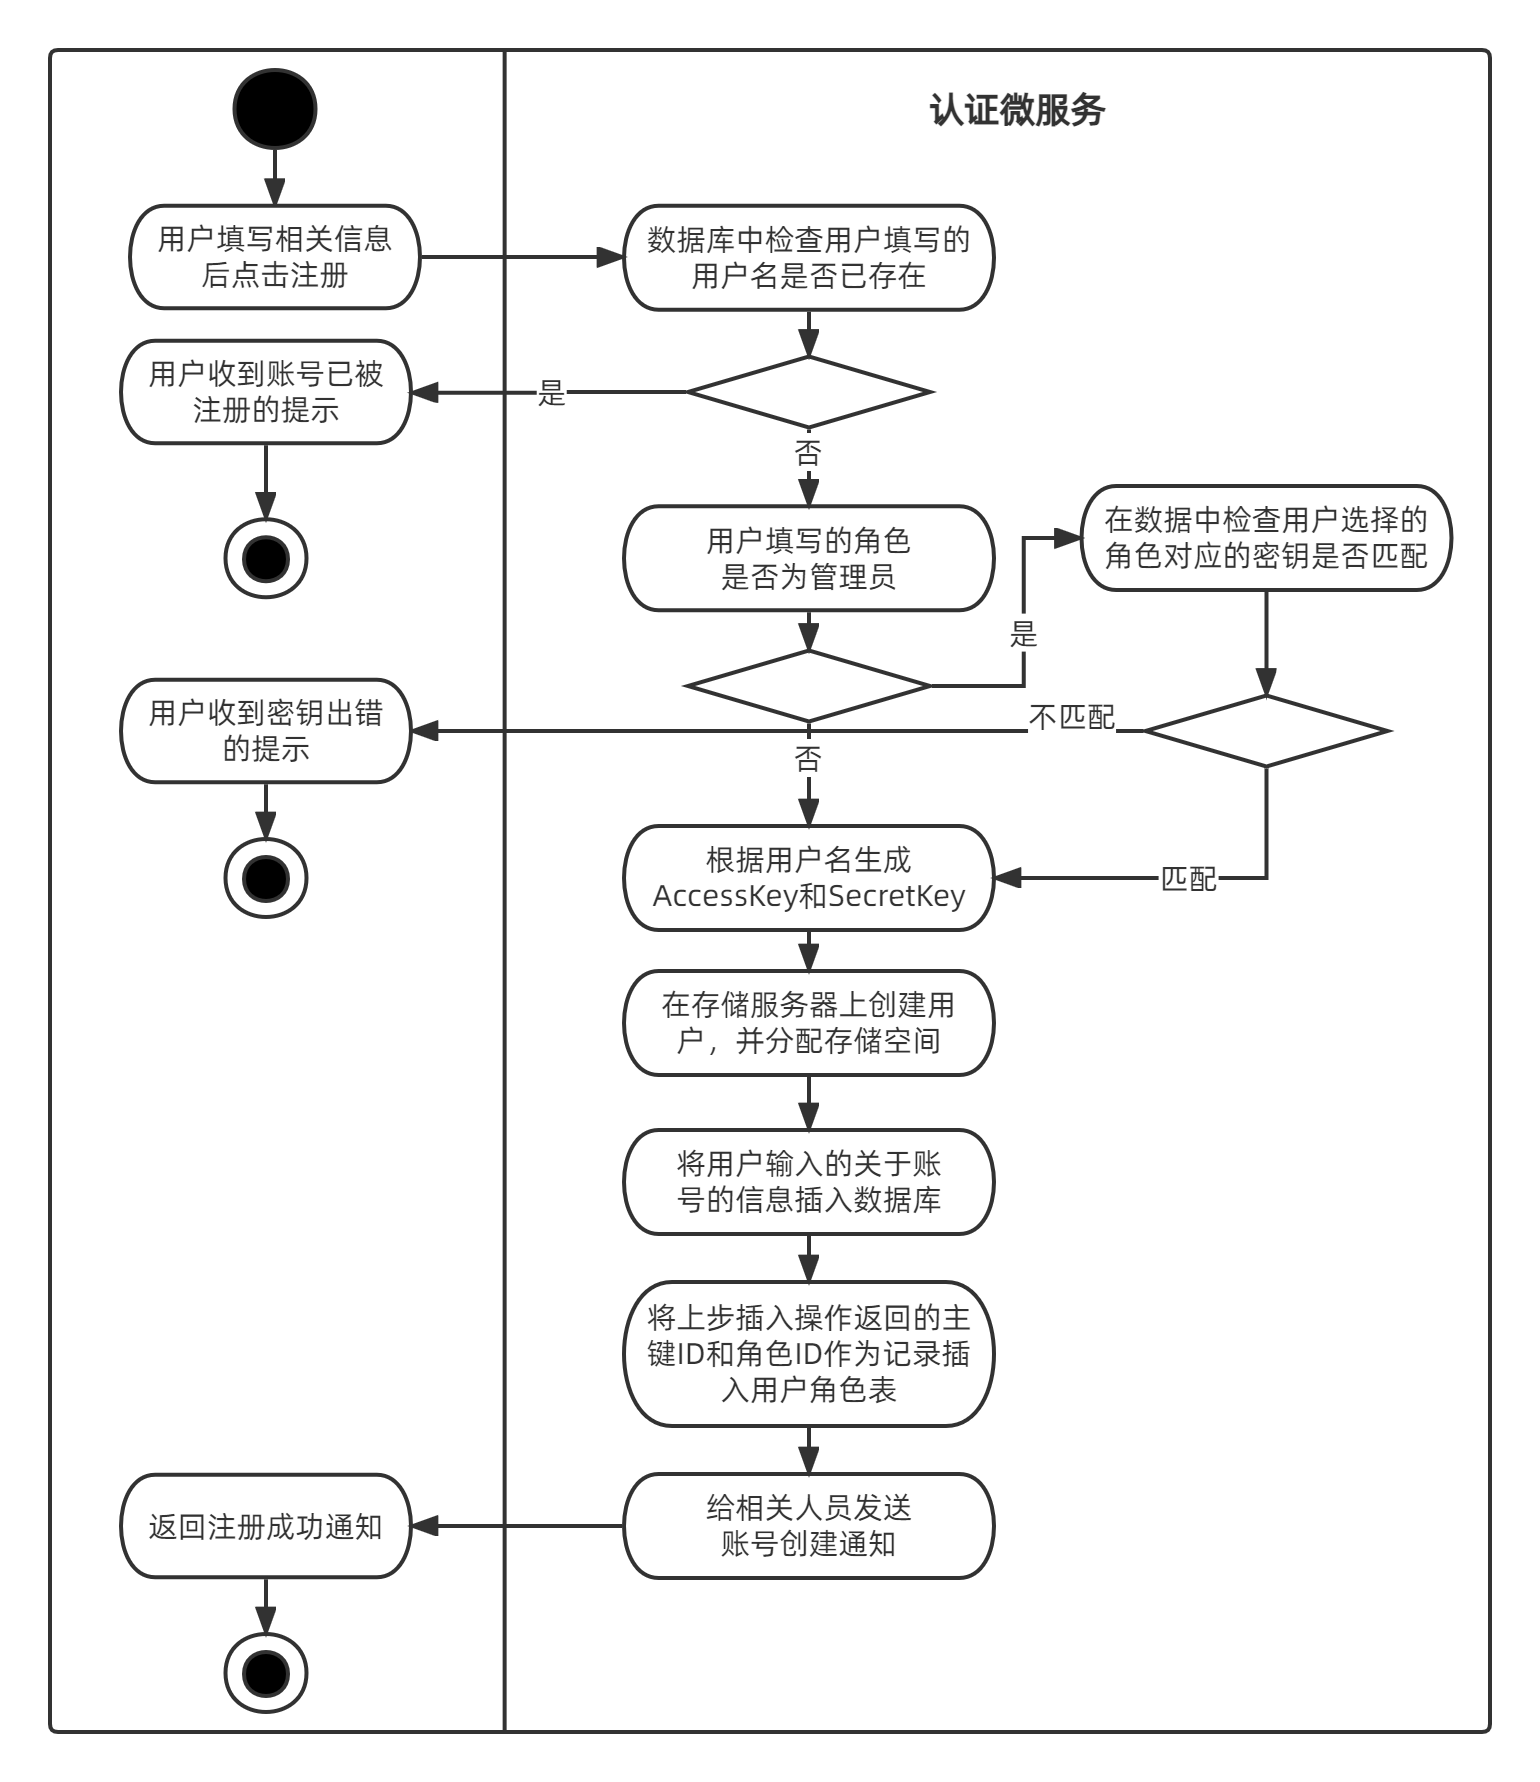
\includegraphics[width=0.8\textwidth]{my_figures/chapter4/用户注册活动图.png}
    \caption{用户注册活动图}
    \label{fig:用户注册活动图}
%     \note{注:图注的内容不宜放到图题中。}
\end{figure}

(2) 密码认证

% 当用户进入存储管理系统的登录页面,并使用已经注册的用户名和密码进行登录时,在登录请求发出后,后端首先会对数据中的用户名进行校验,判断用户名是否存在。如果用户名
% 不存在,后端会向前端返回错误信息。如果用户名存在,会根据选择的hash算法对密码进行hash操作,因为数据库中保存的也是经过hash处理后的密码,之后将进行hash计算后的
% 密码与数据库中的hash值进行匹配,如果成功匹配,则使用相应的算法生成token,否则向前端返回错误信息。密码认证活动图如图\ref{fig:用户名密码认证活动图}所示。

当客户登录存储管理系统的注册网站,并通过自己所登录的用户名和口令完成注册后,当注册申请提交时,系统后端就会对数据中的账户
进行校验,以确定账户的实际存在。如果秘密不存在,后端将向前台传递错误信息。而如果秘密出现,将通过选择的hash方法对秘密进行
hash计算,因为数据库系统中保存的都是已经进行hash处理过的秘密,所以之后将进行hash计算后的秘密和数据库系统中的所有hash数
据进行匹配,一旦实现了配对,将通过相应的方法得到token,否则将由前端反馈错误信息。密码认证的示意图如图四点五中所示。

\begin{figure}[htb]
    \centering
    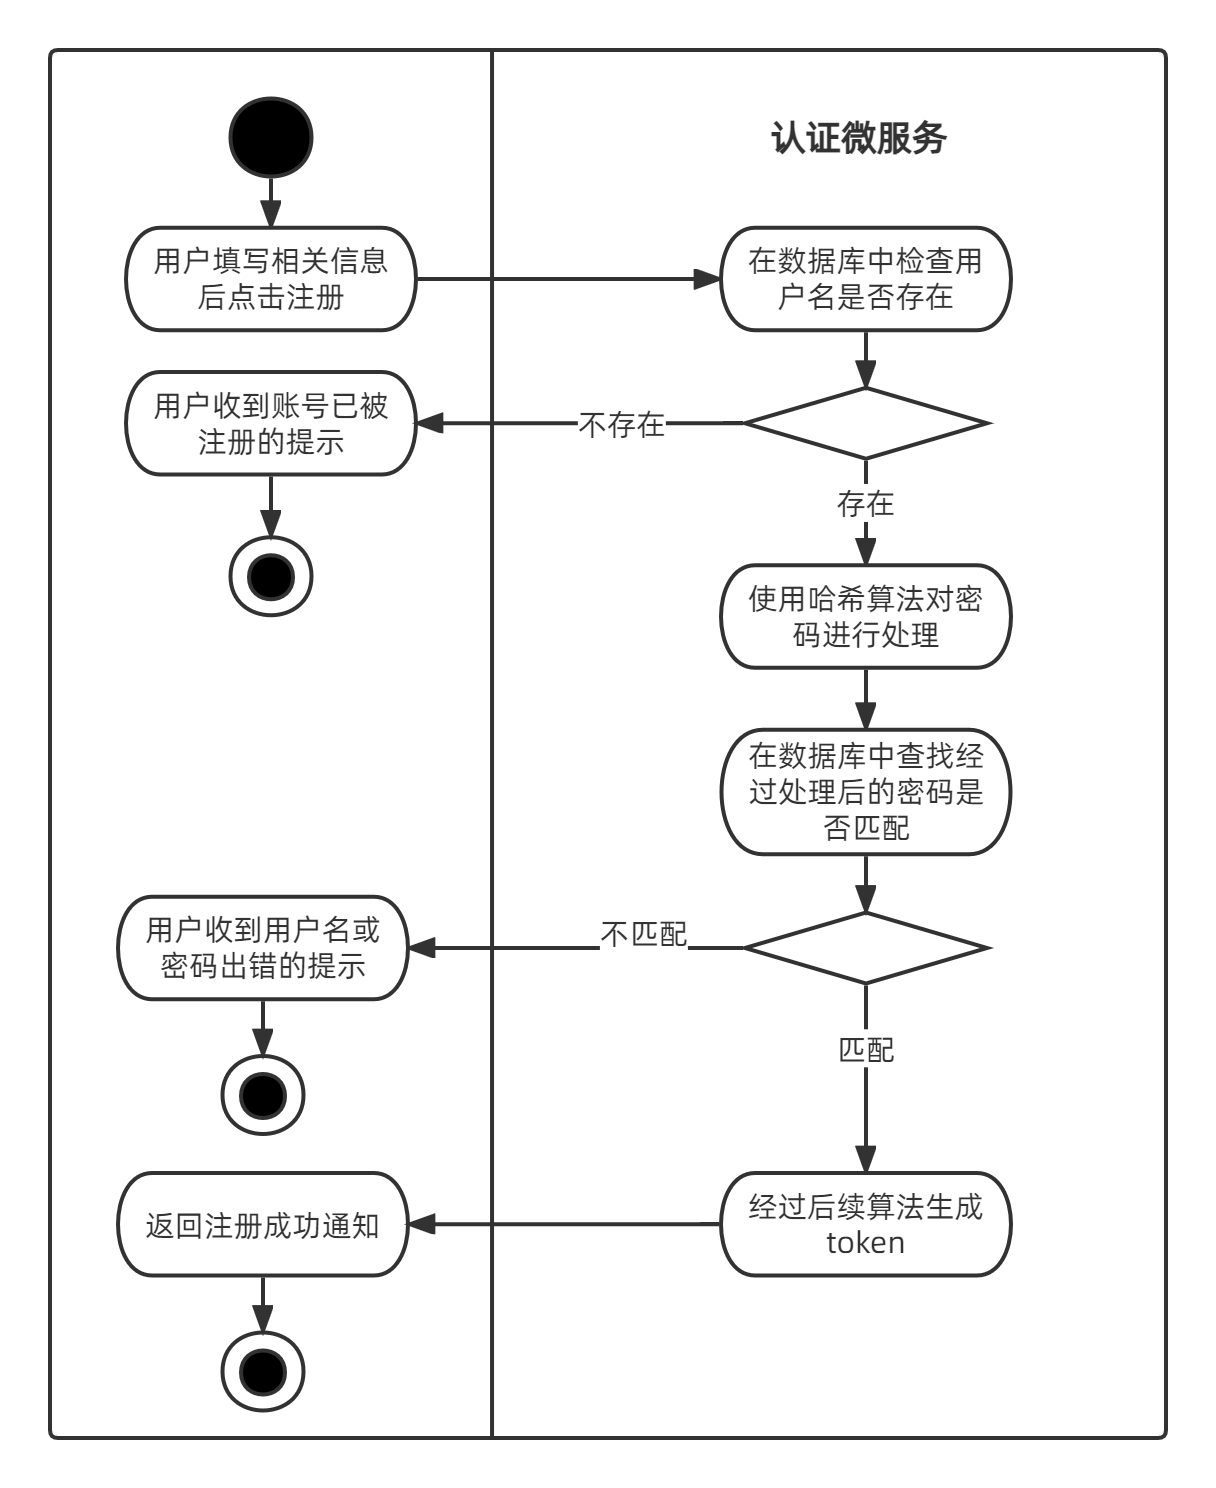
\includegraphics[width=0.8\textwidth]{my_figures/chapter4/用户名密码认证活动图.png}
    \caption{用户名密码认证活动图}
    \label{fig:用户名密码认证活动图}
%     \note{注:图注的内容不宜放到图题中。}
\end{figure}

(3) 颁发令牌

% JSON Web Token 是一个开放标准,为了能在各系统间安全的传输 JSON 信息,它定义了一种数据格式。JWT分别由Header 、 Payload 和Signature这三个英文点号分割的部分
% 共同组成。Header由token的类型和使用的签名算法两部分组成。Payload是JWT的主体部分,主要用来存放业务信息,Payload将发行人、到期时间、JWT编号等七个默认字段提供
% 给开发者选择。同时,用户还可以添加一些需要的自定义字段,比如角色信息和时间戳信息等。由于该部分没有严格的保密处理,所以不能将用户的密码信息构建在该部分。前面
% 两部分被服务器用存储在服务端的私钥进行不可逆的加密算法后,就得到了JWT的第三部分,即签名哈希Signature。Signature的主要防止整个token被篡改,JWT 的 Header 
% 字段会将使用的加密算法记录下来。该私钥应该尽量保证复杂性,以防止当私钥泄漏时,不法分子直接绕过用户名密码的校验,从而利用该私钥随意创建令牌,影响系统安全。
% 颁发令牌活动图如图\ref{fig:颁发令牌活动图}所示。
JSON Web Token是一种开放规范,为了能够在各用户之间可靠的传递JSON数据,它规定了一种新数据格式。JWT分别由Header、
Payload和Signature这三种由英文点所分割的部分所构成。Header主要由token的形式,以及所使用的签名技术二个方面所构成。
Payload也是JWT的基础组成部分,主要用于保存交易数据,Payload中包括发行人、到期日期、JWT编号和七个默认字段提交给开发者
使用。另外,开发者也可加入一些重要的自定义字段,包括角色数据和日期戳数据等。因为该部分并没有经过严格的保密处理,所以无
法直接把整个系统的加密数据都构建在此部分。Signature的功能防止了该token被修改,而JWT的Header字段则将所使用的加密算法全部记
录了下来。颁发令牌活动图如图4.6所示。

\begin{figure}[htb]
    \centering
    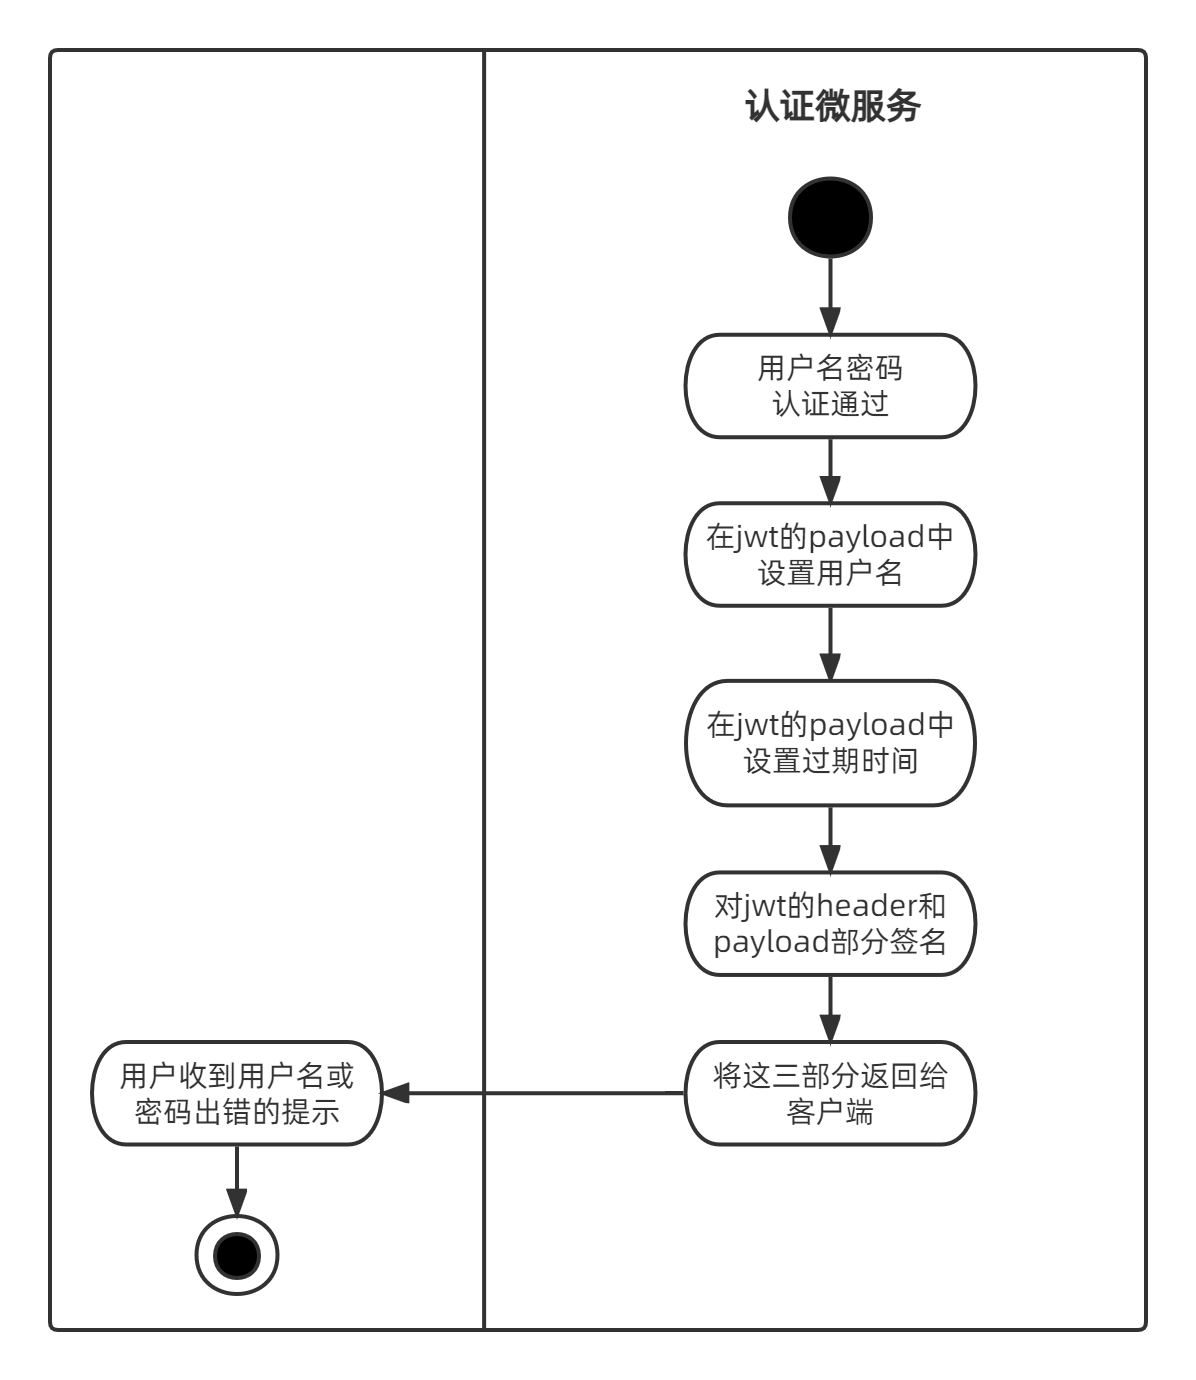
\includegraphics[width=0.8\textwidth]{my_figures/chapter4/颁发令牌活动图.png}
    \caption{颁发令牌活动图}
    \label{fig:颁发令牌活动图}
%     \note{注:图注的内容不宜放到图题中。}
\end{figure}

 

(4) 认证令牌

% 当网关收到用户请求时,调用认证微服务的接口对其携带的token进行验证。 首先,会使用服务器中存储的JWT密钥对 token 的前两部分进行签名,将签名结果与token的第三部分
% 进行比较,如果相同,则通过验证。这个过程主要是为了避免token被篡改,篡改后的token无法通过验证。然后,会对token第二部分中的时间戳进行判断,主要是检查时间戳是否
% 过期,如果时间戳过期,则用户需要重新登录请求token。过期时间可由开发人员灵活设置,但过期时间必须设置的适当,太长或太短都会存在优点和缺点。若过期时间设置的太短,
% 优点是安全性比较好,即使token泄漏,token也会马上失效;缺点是用户需要在很短的时间内反复重新登录,体验极差。若过期时间设置的太长,优点是用户不用频繁重新登录,可
% 长期保持登录状态;缺点是不法分子有了更多的时间进行非法操作。通过认证后,网关会将消息转发给文件存取系统,用户可进行文件的上传和下载等操作。认证令牌活动图如图

这个过程主要是为了避免 token被篡改,篡改后的 token无法通过验证。之后,系统会对token在第二部分中的时间戳做出判断,重点就是检测时间戳有没有过期,一旦时间
戳已经过期,那么用户就必须再次注册并申请token。过期日期也可以由开发人员灵活设定,但过期日期需要设定的适当,太长或太短都
会存在优点和缺点。若将过期日期设定的太短,优点是安全性比较好,即使 token泄漏,token也会马上失效;缺点是用户需要在很短的
时间内反复重新登录,体验极差。如果过期日期设定的较长,好处是客户不必频繁重复注册,可以长期保持注册状态;缺点是不法分子有
了更多的时间进行非法操作。通过认证后,网关会将消息转发给文件存取系统,用户可进行文件的上传和下载等操作。认证令牌活动图
如图4.7所示。

\ref{fig:认证令牌活动图}所示。

\begin{figure}[htb]
    \centering
    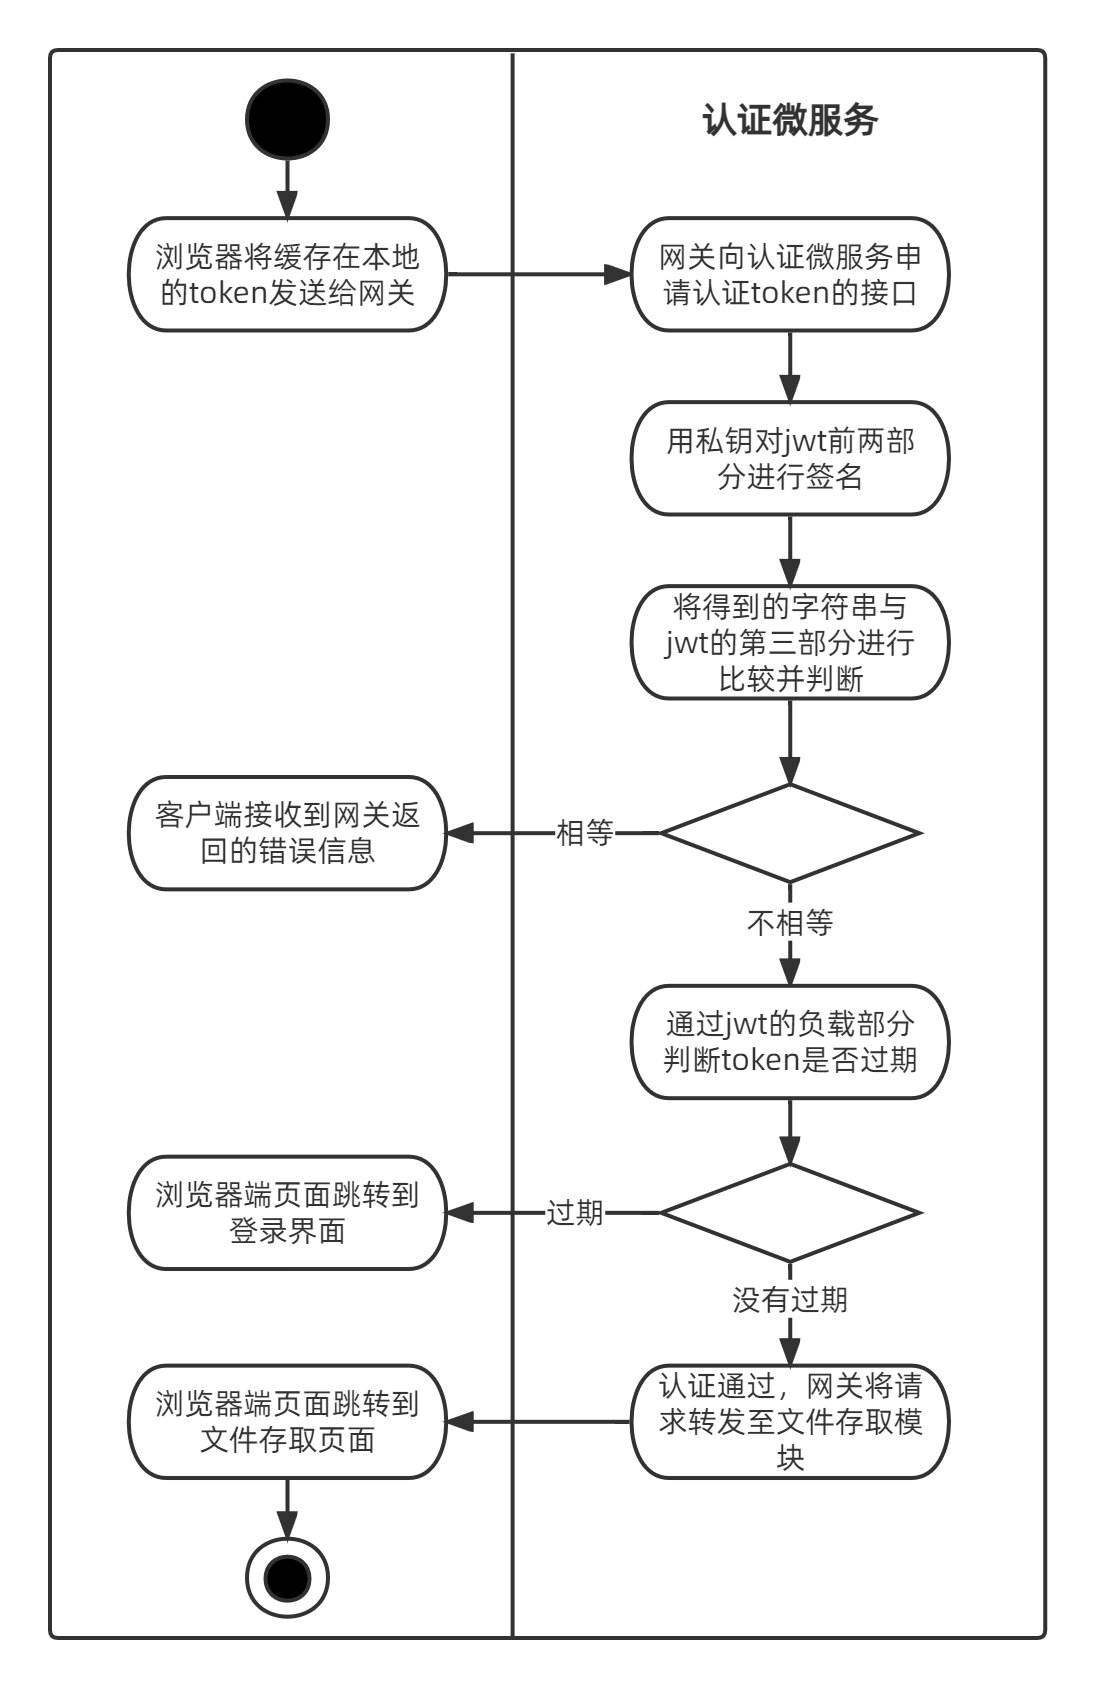
\includegraphics[width=0.8\textwidth]{my_figures/chapter4/认证令牌活动图.png}
    \caption{认证令牌活动图}
    \label{fig:认证令牌活动图}
%     \note{注:图注的内容不宜放到图题中。}
\end{figure}

\subsection{网关鉴权模块}

% 网关鉴权模块是所有微服务的门户,用户发给微服务的所有请求都会首先经过网关,但网关对于客户端来说是完全透明的。网关的主要作用就是为整个系统的安全提供保障,网关会
% 提供所有安全性方面的校验,整个系统将网关的端口作为唯一的入口即可。网关鉴权模块主要由请求转发、请求鉴权和路由发布三个子模块组成。网关鉴权模块的功能结构图如图
% \ref{fig:网关鉴权模块功能结构图}所示。

网关鉴权功能是整个微服的入口,系统发给微服的任何要求都是先通过网关,但网关对于客户端来说是完全透明的。网关的最主要功能
就是为整个系统的安全性提供保护,因为网关会进行各种安全方面的校验,整个操作系统把网关的所有接口都当做唯一的入口即可。网
关鉴权模块主要由请求转发、请求鉴权和路由发布三个种子模型所构成。网关鉴权模型的基本功能结构图,如图四点八所示。

\begin{figure}[htb]
    \centering
    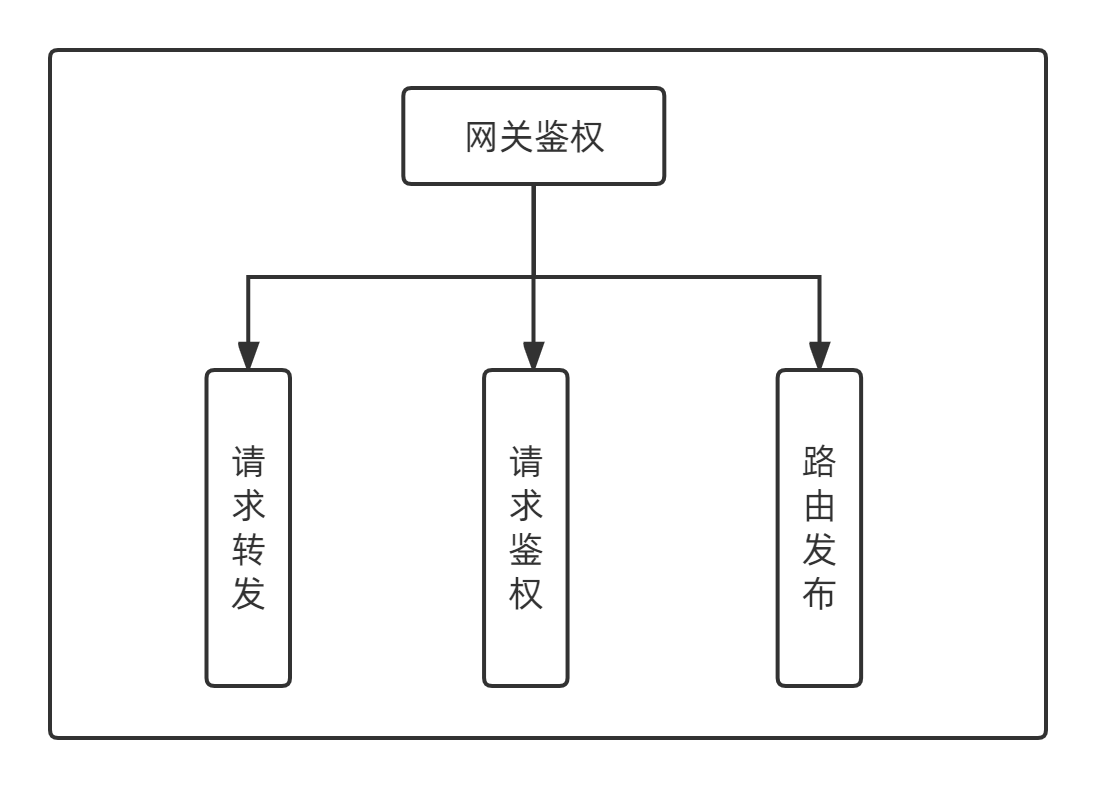
\includegraphics[width=0.8\textwidth]{my_figures/chapter4/网关鉴权模块功能结构图.png}
    \caption{网关鉴权模块功能结构图}
    \label{fig:网关鉴权模块功能结构图}
%     \note{注:图注的内容不宜放到图题中。}
\end{figure}

(1) 请求转发

% 网关根据路由转发请求是网关的基本功能, 用户配置好路由信息后,网关会根据这些路由信息将请求转发给指定的微服务,而且还会判断是否需要应用过滤器。网关配置了四个
% 路由项,第一个是根据用户请求中的/Oauth 字段将请求转发至认证微服务,第二个是根据用户请求中的/policyweb字段将请求转发至策略控制微服务,第三个是是根据用户
% 请求中的/fileweb字段将请求转发至文件存取微服务,第四个是根据用户请求中的/systemweb字段将请求转发至系统维护微服务,并对这些请求应用过滤器,在过滤器中完成
% 检查令牌和校验权限的逻辑。

网关就将按照这个路由信息把请求转送到特定的微服,同时还可以确定是否要使用过滤器。



(2) 请求鉴权

% 网关只会对要转发至策略控制、文件存取和系统维护微服务的请求应用过滤器,在过滤器中通过调用认证令牌子模块的接口检查 token 的正确性,如果检查通过,会调用权限管理
% 模块中的接口,该接口根据token中的用户名来获取用户的权限列表,权限列表中的内容即用户可访问的路径,然后查找用户权限列表判断用户请求中的URI是否存在,如果该路径
% 存在,则说明用户拥有访问该接口的权限,否则没有访问权限,向前端返回错误信息。请求鉴权活动图如图\ref{fig:请求鉴权活动图}所示。

一旦检测通过后,则调用授权管理模块中的入口,该接口通过检查token中的信息就可以得到对用户的
授权信息,权限列表中的内容也就是用户可以访问的途径,然后在使用授权列表中检测用户请求中的URI是否存在,一旦该路径存在,就表
示对其拥有访问的权利接口的权限,否则没有访问权限,给前端返回了错误信息。请求的鉴权活动图,如图四点九所示。

\begin{figure}[htb]
    \centering
    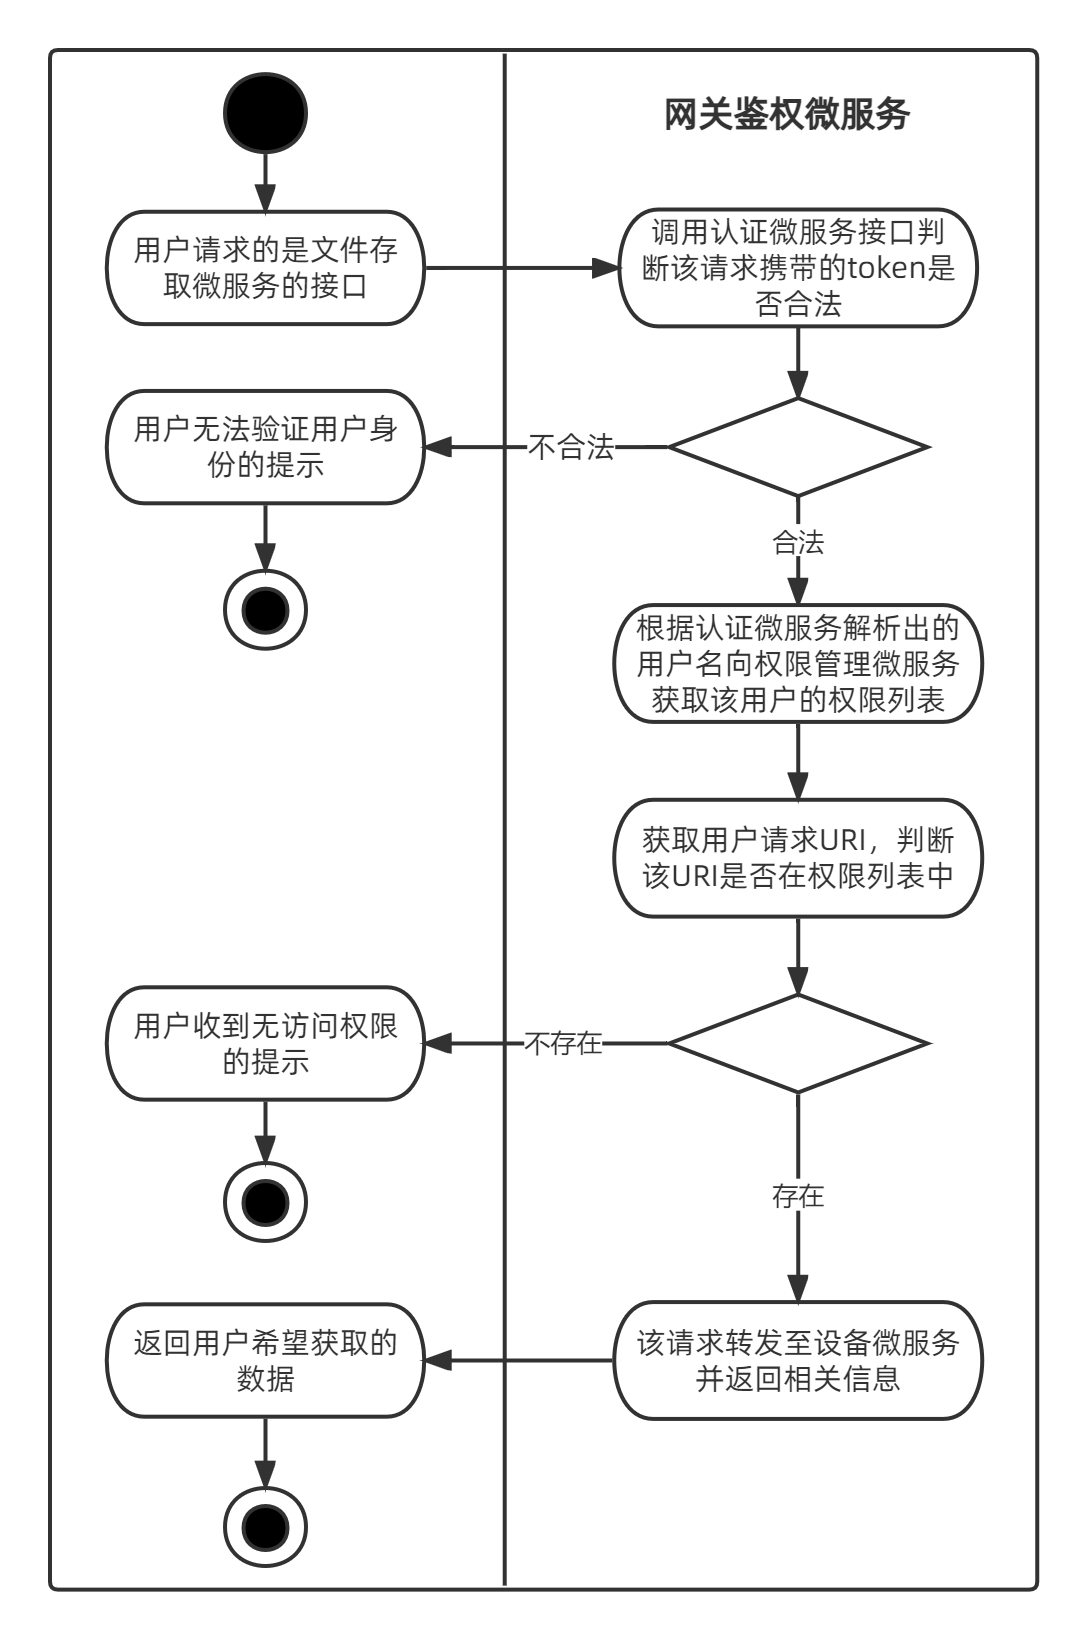
\includegraphics[width=0.8\textwidth]{my_figures/chapter4/请求鉴权活动图.png}
    \caption{请求鉴权活动图}
    \label{fig:请求鉴权活动图}
%     \note{注:图注的内容不宜放到图题中。}
\end{figure}

(3) 路由发布

% 当请求到达网关路由之后,会根据写在项目配置文件中的网关路由转发请求,这些配置文件会在项目启动的时候被加载,但这种方式存在着很大的问题。当我们在配置文件中修改
% 路由项之后需要对项目进行重启,这将耗费极大的运维成本。所以我们可以采用Spring Cloud Gateway 提供的另外一种加载路由信息的方式,该方式可以在项目正常运行的情况xi
% 下,动态的在内存中加载路由信息,在这里采用了Redis,redis通过阻塞获取消息的方式来确定是否有新的路由项要发布,权限控制模块作为Redis中的生产者,该模块负责路由的
% 更新和发布,并且将消息发送至Redis。

在申请到网关路由后,就会通过将写入到项目配置文件中的网关路径转发申请,而这种配置文件通常会在项目刚启动的时候就被载入,
但是这个方法也面临了很多的问题。如果我们在系统配置文件中更改路由项之后就需要对项目进行重启,这将耗费极大的运维成本。
所以我们也可以使用在Spring Cloud Gateway中的另一个载入路由消息的方法,在这种方式能够保证项目正常工作的前提下。

\subsection{权限控制模块}

% 权限控制模块的主要作用是系统管理员用来管理用户账号、角色、权限以及网关路由。权限控制模块主要包含三个子模块,分别是账号角色权限管理子模块,角色分配子模块和网关
% 路由管理子模块。账号角色权限管理主要负责对账号角色以及权限的数据进行管理,角色分配主要负责将账号与角色、角色与权限进行关联,处理这三者之间的分配关系。网关路由
% 管理主要负责对网关路由的数据进行管理以及对消息队列Redis进行发布。权限控制模块的功能结构图如图\ref{fig:权限控制模块功能结构图}所示。

权限控制模块的主要功能,是系统管理员用来管理的用户帐号、角色、授权和网关路由。授权管理模块主要包括三个种子模块,分别为
帐号角色授权管理子模块,角色分配子模块和网关路由管理子模块。帐号角色授权管理主要负责对帐号角色及其授权者的数据进行管理,
角色分配主要负责将帐号与角色、角色和权限进行关联,并管理这三方间的分配关系。而网关路由管理则主要负责对经过网关路由的数
据进行管理,和对消息队列Redis进行发布。权限管理模型的功能结构图,如<br>图四点一零中所示。

\begin{figure}[htb]
    \centering
    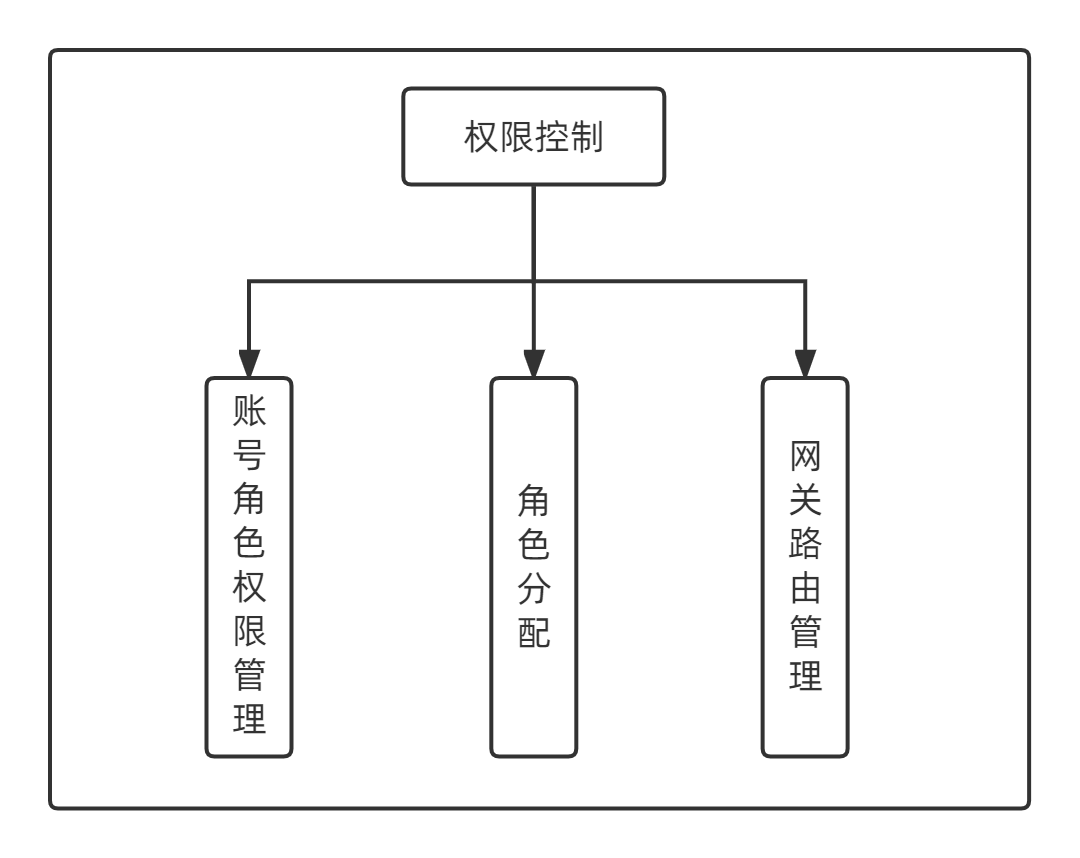
\includegraphics[width=0.8\textwidth]{my_figures/chapter4/权限控制模块功能结构图.png}
    \caption{权限控制模块功能结构图}
    \label{fig:权限控制模块功能结构图}
%     \note{注:图注的内容不宜放到图题中。}
\end{figure}

(1) 账号角色权限管理

% 账号角色权限管理主要是负责管理用户账号、角色以及权限等数据。可以对这些信息进行常规的操作,比如增加、删除、修改和查看。用户账号信息主要包括用户名、密码以及邮箱
% 等信息。系统中的角色主要有超级管理员、普通管理员和普通用户这三种。权限指的是用户访问接口的权限,系统中每一个接口都对应一个访问路径,拥有某接口的访问权限本质上
% 就是拥有其访问路径。

帐号角色授权管理中心主要是负责管理玩家帐号、人物的授权等信息。可对一些数据进行常规的操作,包括添加、移除、修改和查看。
用户账号信息,主要包含了用户名、密码以及邮箱等信息。系统中的管理者,一般包括超级管理者、正常使用者和一般使用者这三类。
权限说的是系统访问连接的权利,系统的每一条连接只对应一条的路径,拥有某接口的访问权限本质上就是拥有其访问路径。

(2) 角色分配

% 角色分配主要负责将用户和权限与角色绑定在一起,给用户绑定一个角色,就相当于给员工安排一个职位,给角色绑定权限,就相当于给职位授予一定的权限。为了维护这两种关联
% 关系,分别设计了用户角色关联表和角色权限关联表。用户角色关联表的记录由用户ID和角色ID构成,角色权限关联表中的记录由角色ID和权限ID构成。管理员在将角色分配给用户
% 和权限时,可能同时存在绑定和解绑两种操作,在实现时需要对这个操作进行数据库的事务控制,如果在事务处理的过程中发生了错误,可以及时对操作进行回滚。

角色分配系统主要负责把用户和权限与角色捆绑在一起,给用户绑定一个角色,就等于为员工设置了一种职务,给人物绑定权限,就等于为
职位授予了相应的权利权限。为保护这二个关联关系,公司分别设计了用户角色关联表和人物权限关联表。用户角色关系表的记录由使
用者ID和人物ID组成,人物授权关系表中的记录则由人物ID和授权ID组成。管理员在把人物信息分享给使用者和授权时,就可以同时存
在绑定和解绑二种操作,在实现时必须对这种操作实施数据库的事务管理,一旦在事务处理的过程中出现了出错,就可以及时地对操作进
行回滚。

(3) 网关路由管理

% 网关路由管理主要负责对网关路由信息进行增加、删除、修改和查看操作,以及网关鉴权模块进行通信。在管理员将组成路由的一些必要信息保存在数据库中后,网关鉴权模块无法
% 感知这一操作,只有当管理员将路由信息发布之后,此时系统会向Redis发布一条信息,该消息由数据库中所有网关路由的信息组成,然后被网关鉴权模块获取,并抽象成内存中的
% 网关路由对象进行发布。网关路由模块的主要任务是辅助网关鉴权模块完成动态发布网关路由的功能。 网关路由管理活动图如图\ref{fig:网关路由管理活动图}所示。

网关路由管理系统主要是通过对网关路由数据的添加、删除、更改和查询管理,并通过网关鉴权功能实现路由。但当用户将组成路由的
一些必要数据存储到数据库系统中时,网关鉴权系统并不能感知这一信息,而只是在用户将路由数据发送后,此时操作系统才会向Redis
发出一个消息,该消息由数据库系统中的网关路由的数据构成,随后再由网关鉴权功能收集信息,并抽象为系统内存中的网关路由数据并
加以发布。网关路由系统的主要工作,是帮助网络的鉴权系统实现动态的网关路由的活动。网关路由的过程图,如图四点一一所述。

\begin{figure}[htb]
    \centering
    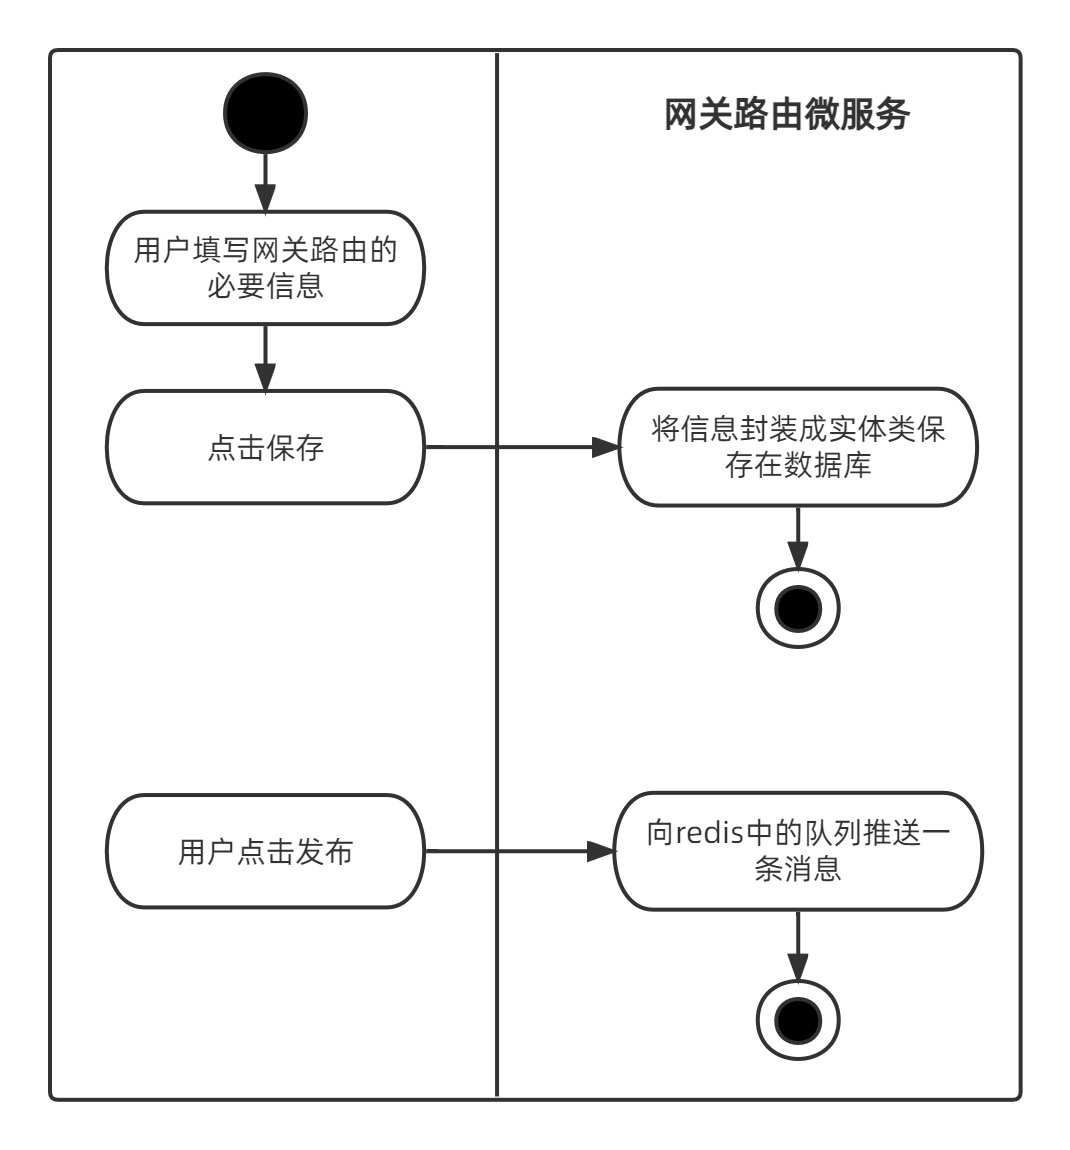
\includegraphics[width=0.8\textwidth]{my_figures/chapter4/网关路由管理活动图.png}
    \caption{网关路由管理活动图}
    \label{fig:网关路由管理活动图}
%     \note{注:图注的内容不宜放到图题中。}
\end{figure}

\subsection{策略控制模块}

策略控制模块主要负责对注册在存储服务器上的用户、分组和访问策略进行管理。策略控制模块主要包含四个子模块,分别是用户管理子模块,分组管理子模块,策略管理子模块和
策略分配子模块。用户管理子模块主要负责对存储用户的相关数据信息进行管理,分组管理子模块主要负责对存储分组的相关数据信息进行管理,策略管理子模块主要负责对访问策
略的相关数据信息进行管理,策略分配主要负责将策略与用户、策略与分组进行关联,处理这三者之间的分配关系。策略控制模块功能结构如图\ref{fig:策略控制模块功能结构图}
所示。

\begin{figure}[htb]
    \centering
    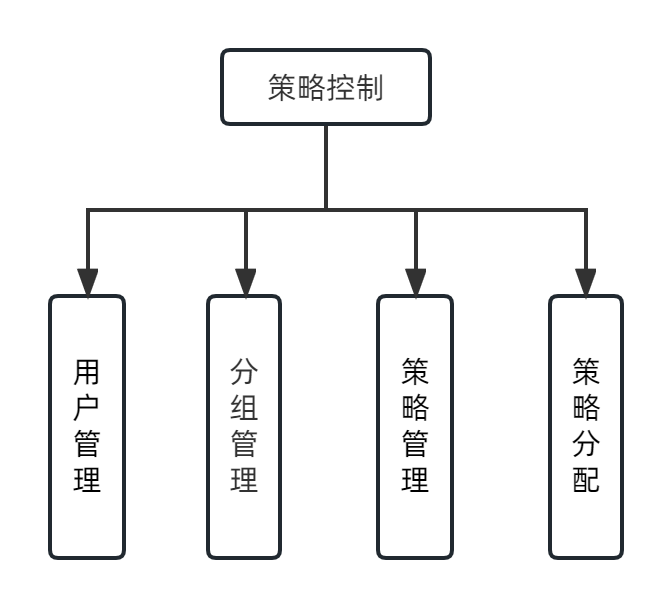
\includegraphics[width=0.8\textwidth]{my_figures/chapter4/策略控制模块功能结构图.png}
    \caption{策略控制模块功能结构图}
    \label{fig:策略控制模块功能结构图}
%     \note{注:图注的内容不宜放到图题中。}
\end{figure}

(1) 用户管理

用户管理主要负责对存储服务器用户账号信息进行数据管理。可以对用户进行增加、删除、修改、查看和禁用操作。存储服务器用户账号主要包括用户名、密码、策略、申请
容量、已用容量等信息。其中,用户名、密码等信息与管理平台用户是相同的,存储服务器用户与管理平台用户的主要区别在于二者所处的位置不同,存储服务器用户创建在存储
服务器上,对相关信息的操作也是直接在存储服务器上生效,而管理平台用户创建在管理系统的后台服务器上,对相关信息的操作是在MySQL数据上生效,并且管理平台用户所包
含的仅为用户的基本信息,存储服务器用户则包含与存储使用情况有关的额外信息。用户管理活动图如图\ref{fig:用户管理活动图}所示。

\begin{figure}[htb]
    \centering
    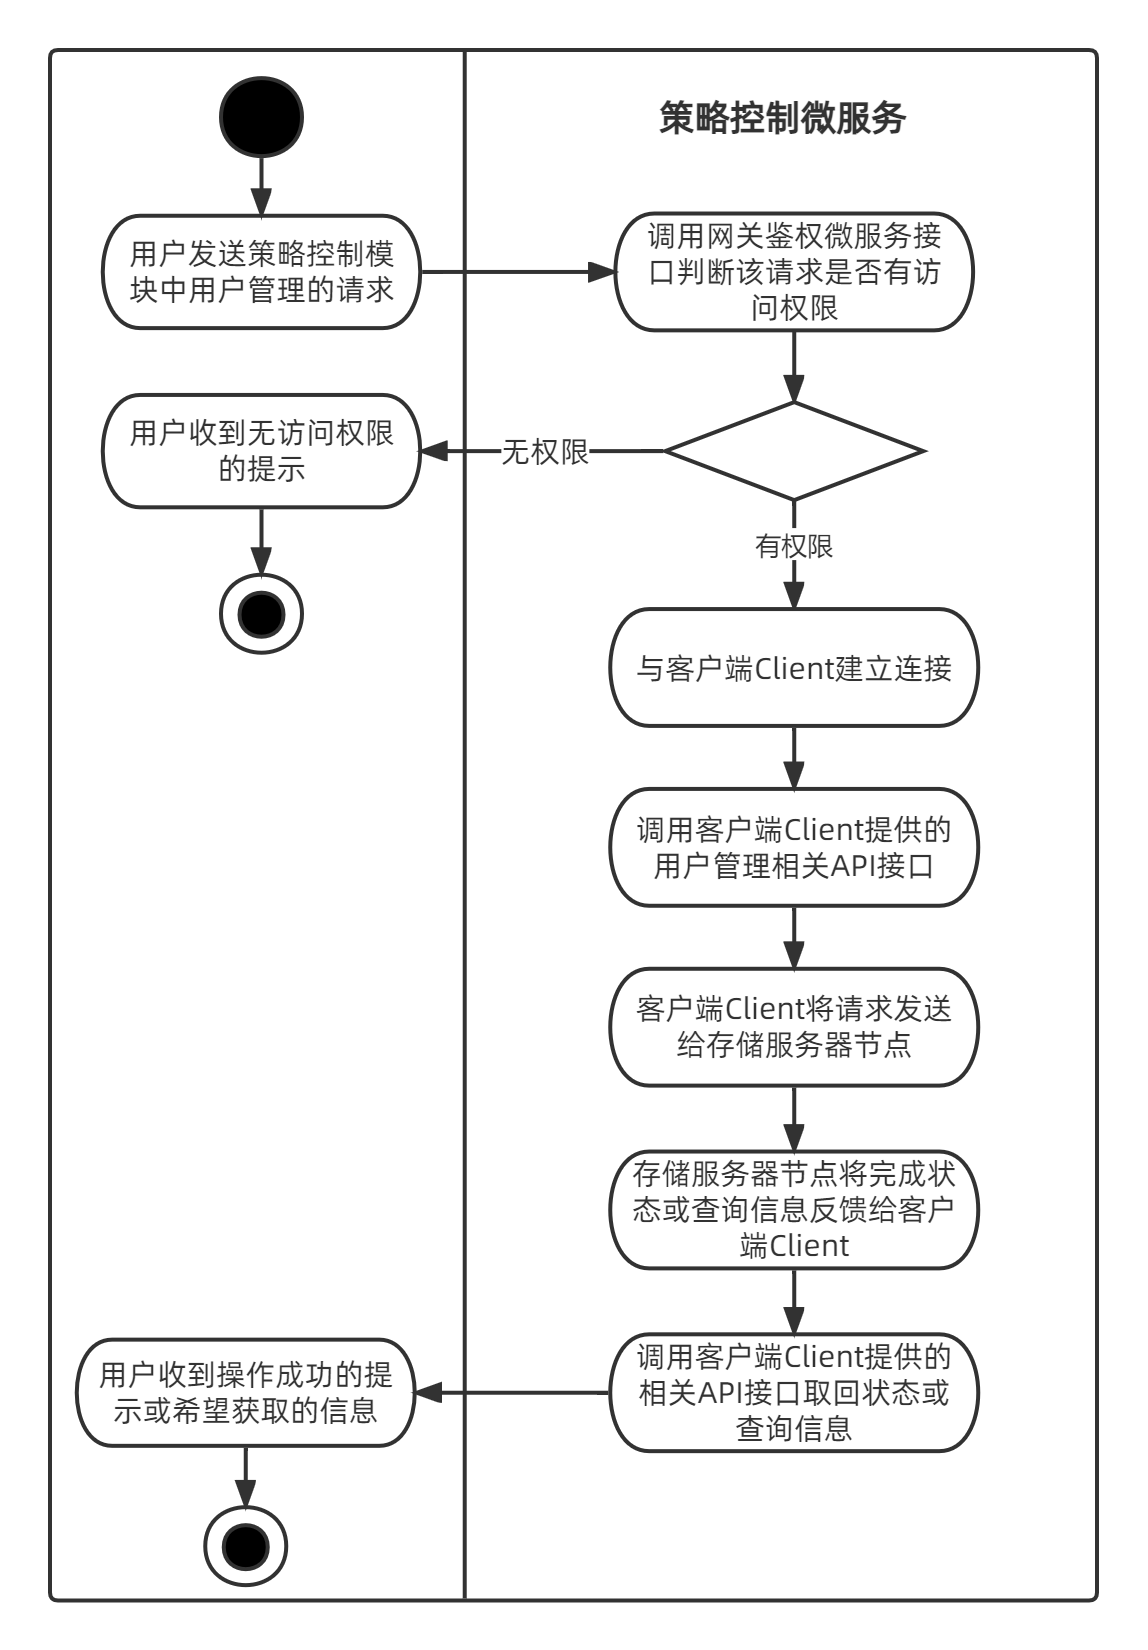
\includegraphics[width=0.8\textwidth]{my_figures/chapter4/用户管理活动图.png}
    \caption{用户管理活动图}
    \label{fig:用户管理活动图}
%     \note{注:图注的内容不宜放到图题中。}
\end{figure}

(2) 分组管理

分组管理主要负责存储服务器分组信息进行数据管理。可以对分组进行增加、删除、修改、查看和禁用操作。存储服务器分组主要包括分组名称、访问策略、是否禁用和创建时间
等信息。当系统发出对分组管理模块的使用申请时,首先会使用网关鉴权微服务进行鉴权,如果没授权,会向前端反馈错误的信息,如果有授权,则与客户端client建立连接,并
调用客户端Client提供的API接口,由客户端Client将请求发送给存储服务器节点,待存储服务器处理结束后,会将完成状态或查询信息反馈给客户端Client,管理系统调用客户
端Client提供的API取回状态或查询信息,并反馈给前端。分组管理活动图如图\ref{fig:分组管理活动图}所示。

% \begin{figure}[htb]
%     \centering
%     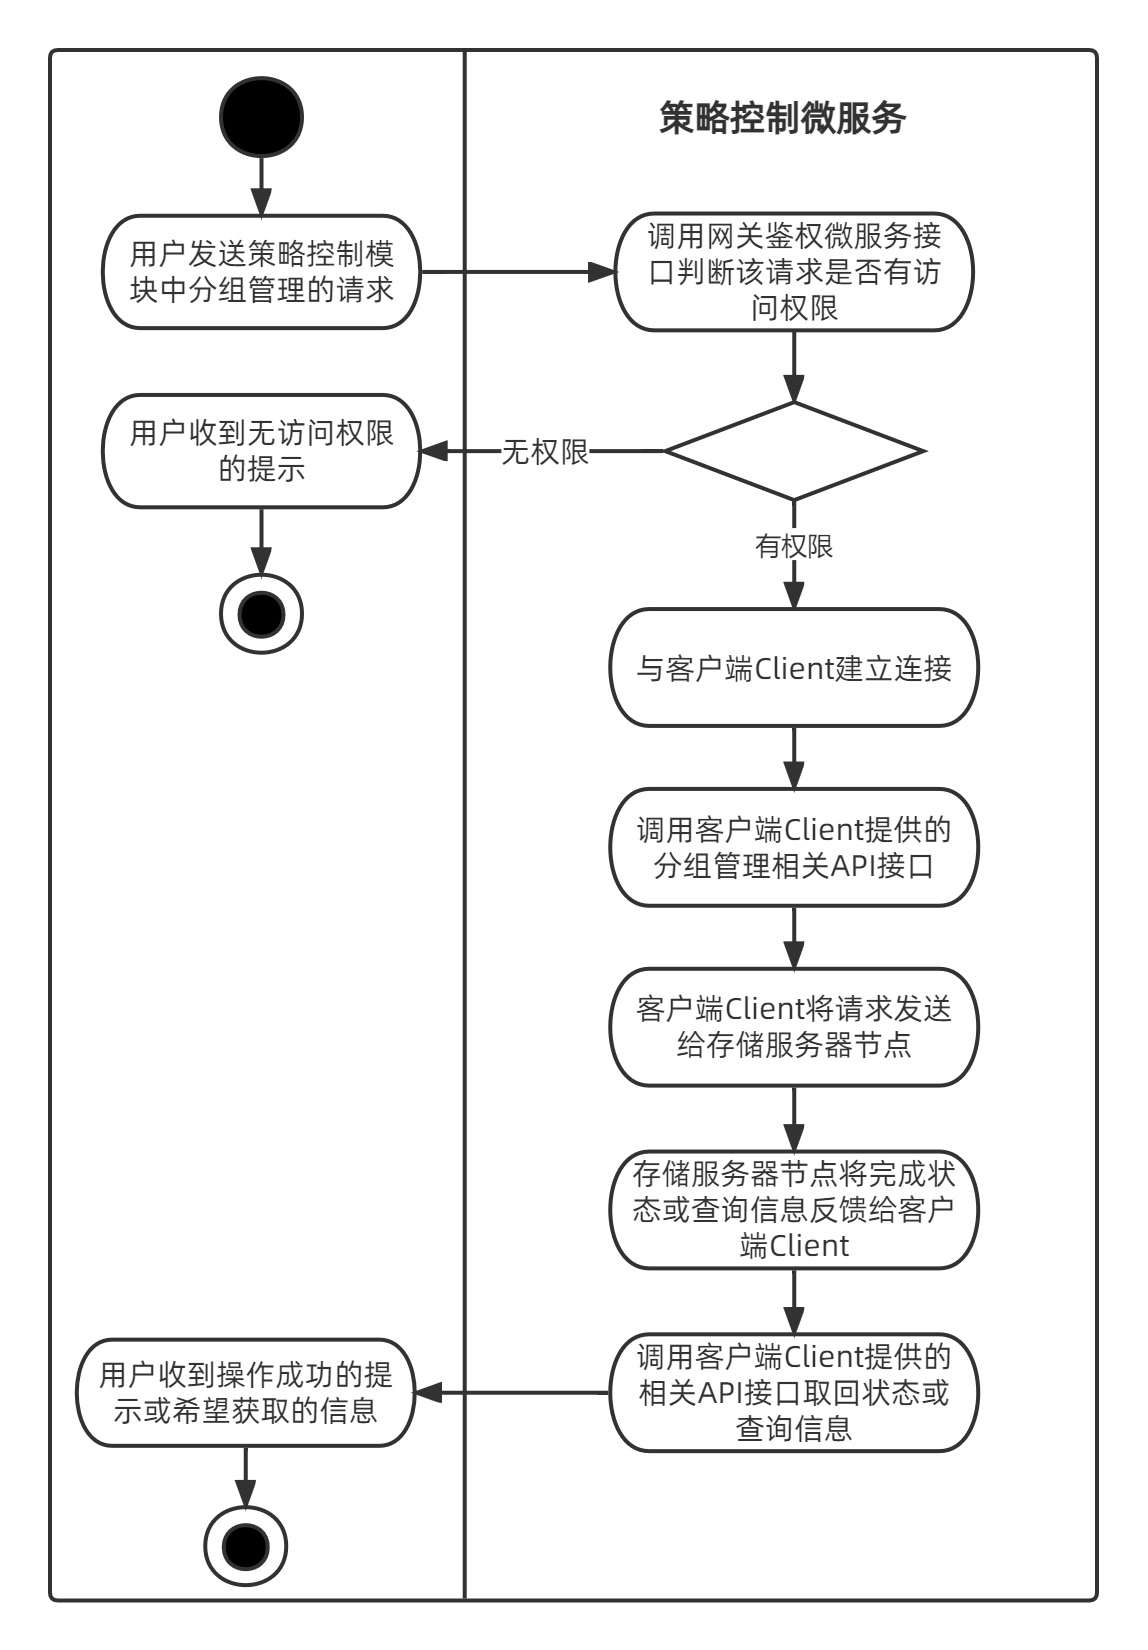
\includegraphics[width=0.8\textwidth]{my_figures/chapter4/分组管理活动图.png}
%     \caption{分组管理活动图}
%     \label{fig:分组管理活动图}
% %     \note{注:图注的内容不宜放到图题中。}
% \end{figure}

(3) 策略管理

分组管理主要负责存储服务器访问策略信息进行数据管理。可以对策略进行增加、删除、修改、查看操作。访问策略主要是针对用户和分组在访问其他用户的Bucket和文件时进行
权限限制,存储服务器已经内置了几种常用的访问策略,管理员可以根据需要自定义创建新的策略,在创建新的策略时,需要配置相关的json文件,该文件包含新策略的实际内容。
除创建新策略以外的其他操作流程与用户、分组管理的操作基本一致。策略管理活动图如图\ref{fig:策略管理活动图}所示。

\begin{figure}[htb]
    \centering
    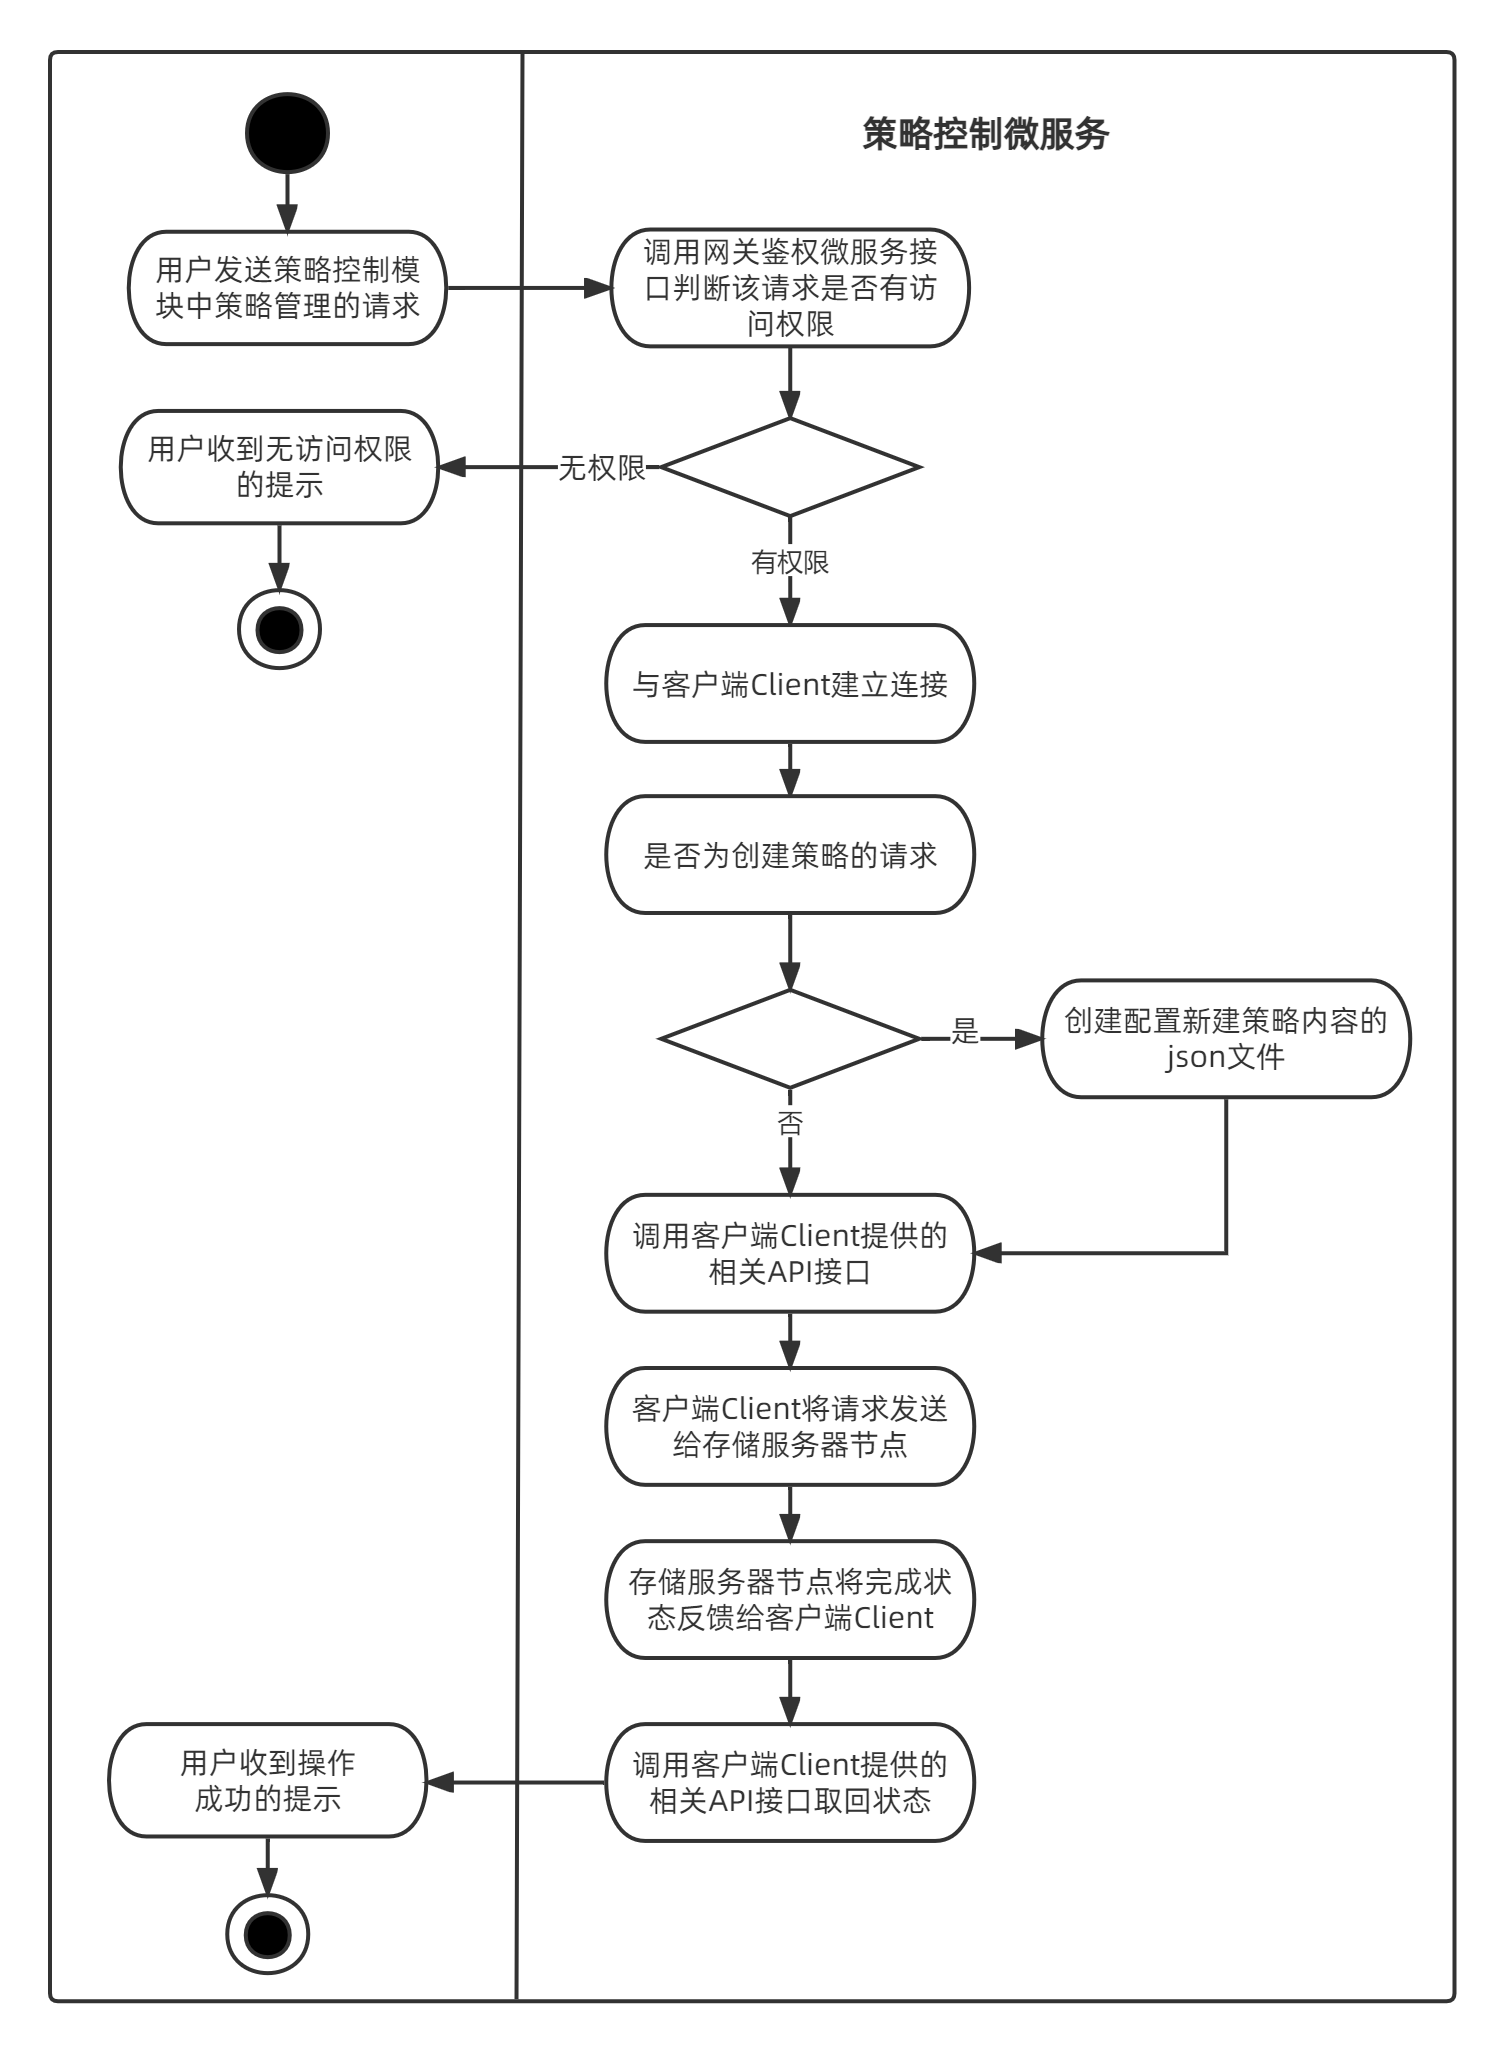
\includegraphics[width=0.8\textwidth]{my_figures/chapter4/策略管理活动图.png}
    \caption{策略管理活动图}
    \label{fig:策略管理活动图}
%     \note{注:图注的内容不宜放到图题中。}
\end{figure}

(4) 策略分配

策略分配主要负责将策略与用户、策略与分组绑定在一起,基本原理和前面的角色分配差不多,用户的访问策略最终由其所在分组的访问策略和其自身的访问策略共同决定。策略
策略分配的操作过程与前面模块基本一致。分配活动图如图\ref{fig:策略分配活动图}所示。

\begin{figure}[htb]
    \centering
    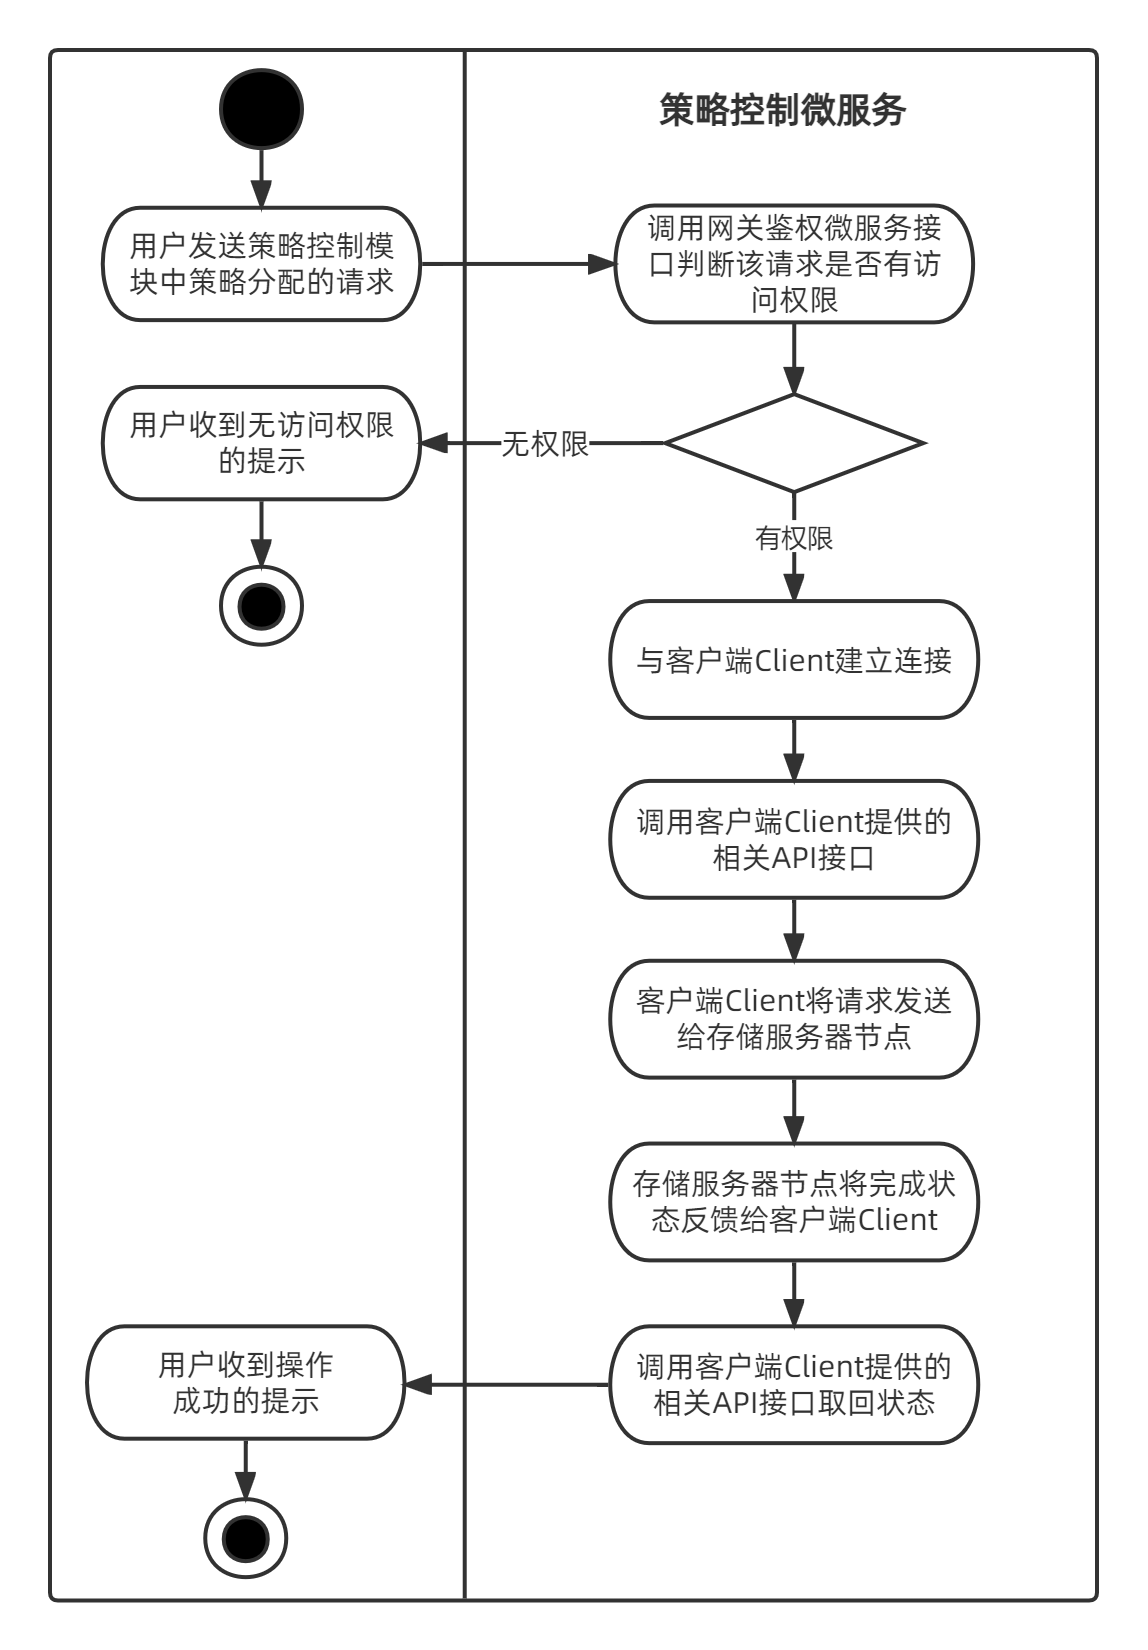
\includegraphics[width=0.8\textwidth]{my_figures/chapter4/策略分配活动图.png}
    \caption{策略分配活动图}
    \label{fig:策略分配活动图}
%     \note{注:图注的内容不宜放到图题中。}
\end{figure}

\subsection{文件存取模块}

% 文件存储模块是本系统最核心的模块,也是普通用户访问最频繁的模块,该模块主要分为四个子模块,分别是桶管理子模块、文件上传子模块、文件下载子模块和文件删除子模块。
% 文件存取模块功能结构图如图\ref{fig:文件存取模块功能结构图}所示。

文件存储模块是本系列中最基础的功能,同时也是普通用户访问最常见的功能,该系统目前包括了四大子模块,分别为桶管理子模块、
文件上传子模块、文件加载子模块和文件删除子模块。文件存取模块功能的结构图如图四点一六所述。

\begin{figure}[htb]
    \centering
    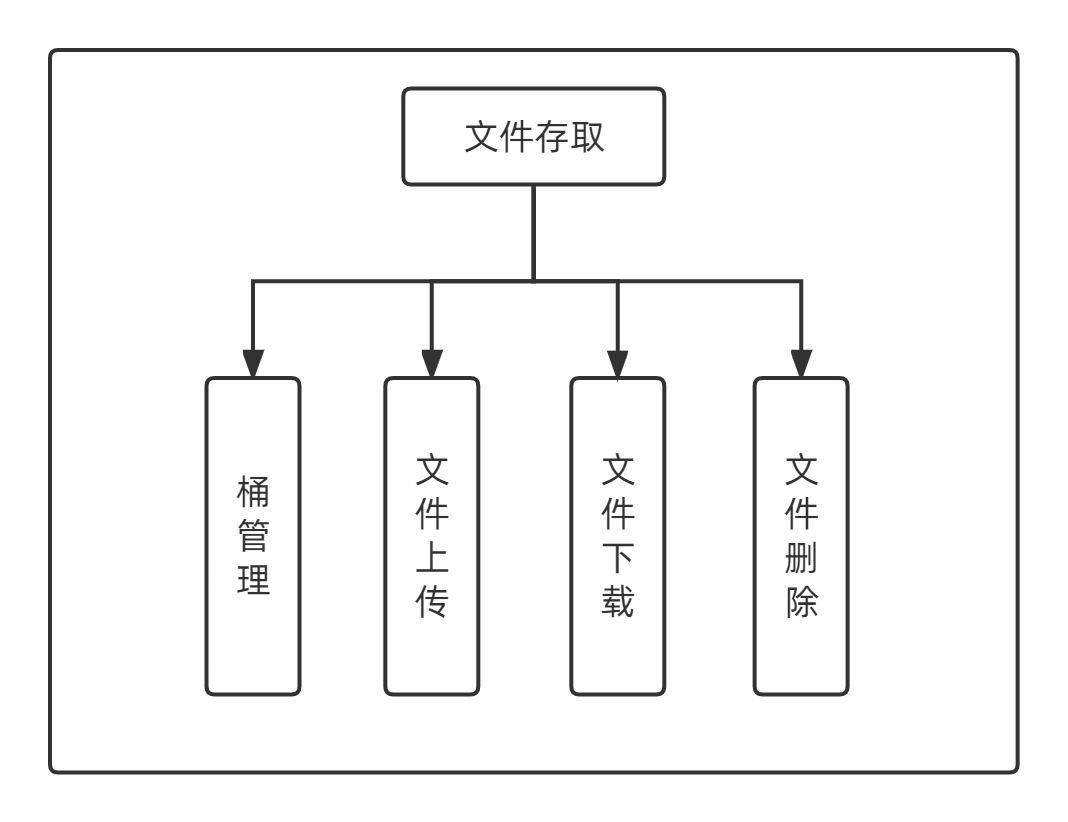
\includegraphics[width=0.8\textwidth]{my_figures/chapter4/文件存取模块功能结构图.png}
    \caption{文件存取模块功能结构图}
    \label{fig:文件存取模块功能结构图}
%     \note{注:图注的内容不宜放到图题中。}
\end{figure}

(1) 桶管理

桶管理模块主要负责对用户的存储桶进行管理。可以对用户的存储桶进行增加、删除、修改、查看操作,但操作的前提是用户拥有对应的访问策略,比如用户对桶的访问策略是只读,
那么该用户将只能对桶进行查看,无法进行修改、删除等其他操作。对桶进行删除操作时,需要在桶里的文件全部被删除之后方可进行,即只可删除空桶。这里的用户不仅指普通用户,还包括普通管理员。
当对木桶进行非创建性操作时,必须首先确定木桶是否存在,若桶不存在,将向前端反馈错误的信息。
% 在对桶进行非创建操作时,需要先判断桶是否存在,如果桶不
% 存在,则向前端反馈错误信息。桶管理活动图如图所示。

% \begin{figure}[htb]
%     \centering
%     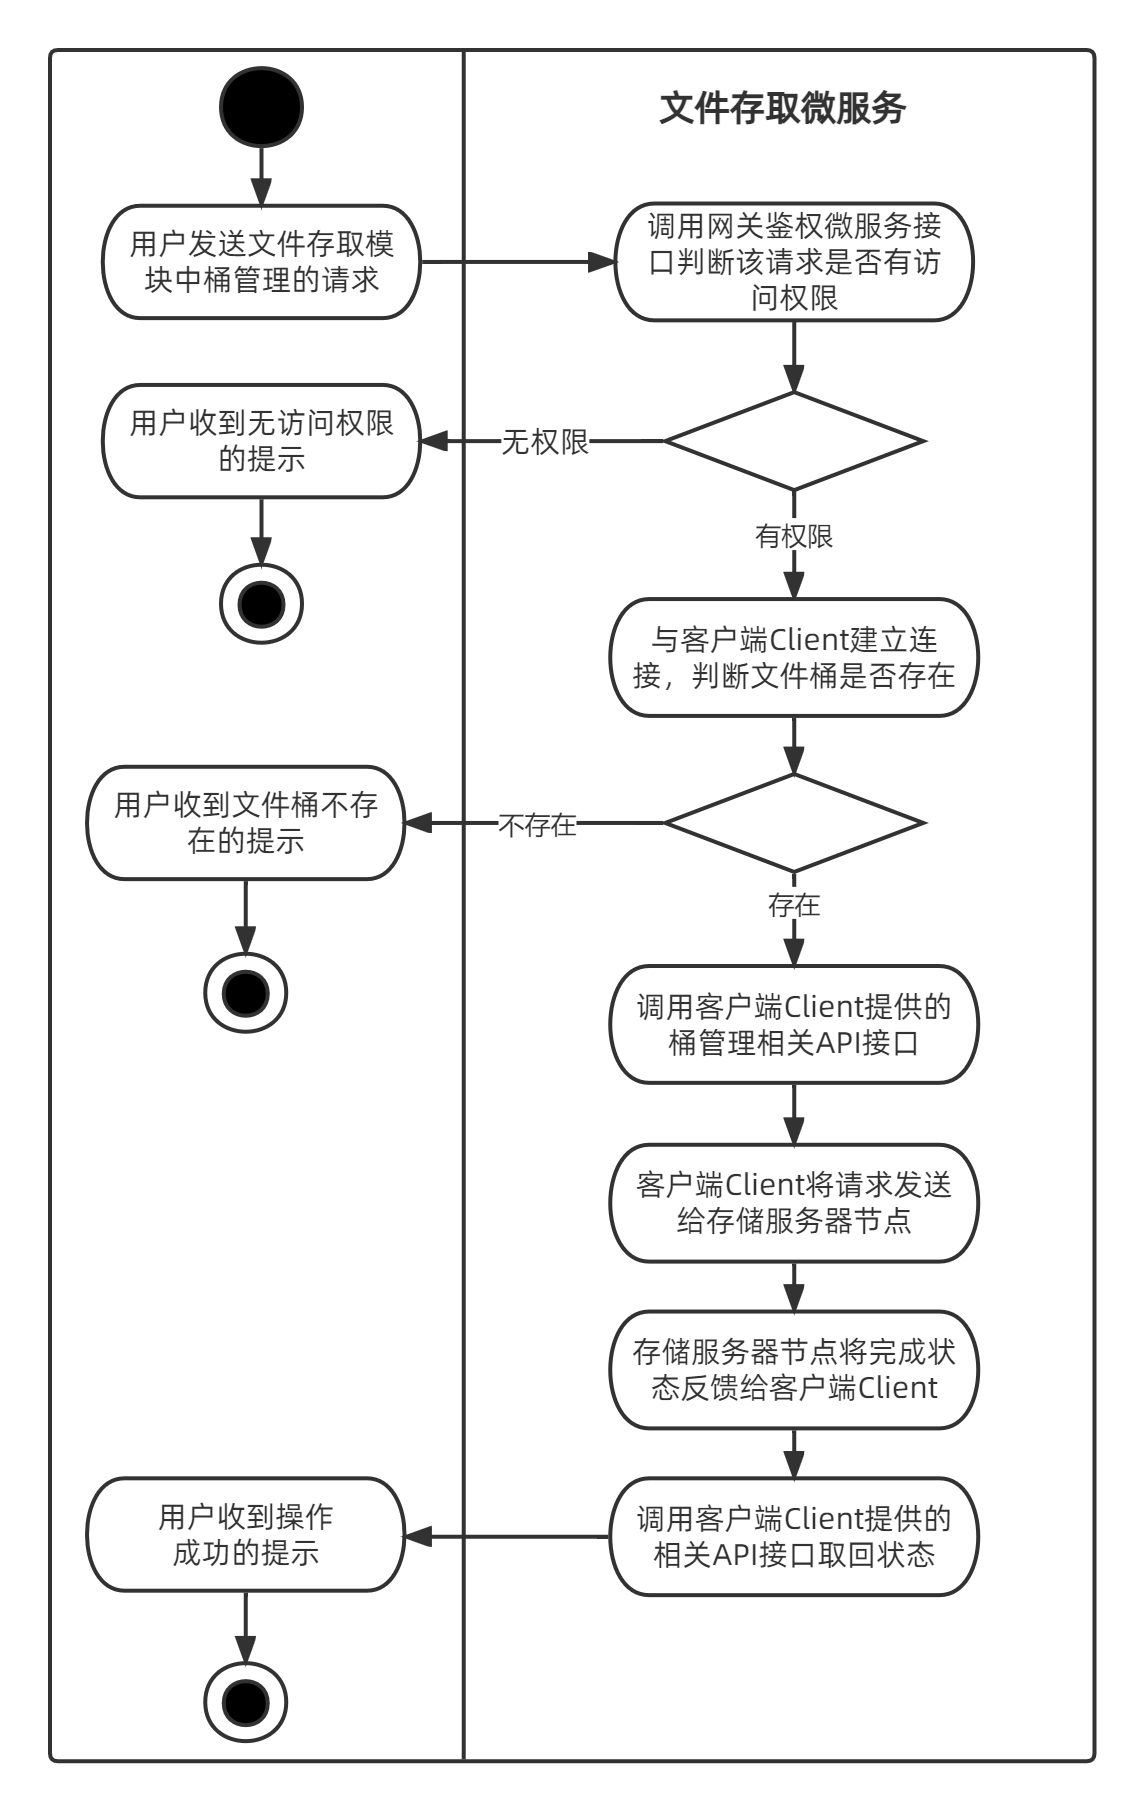
\includegraphics[width=0.8\textwidth]{my_figures/chapter4/桶管理活动图.png}
%     \caption{桶管理活动图}
%     \label{fig:桶管理活动图}
% %     \note{注:图注的内容不宜放到图题中。}
% \end{figure}

(2) 文件上传

% 文件上传模块主要负责将用户的文件上传至数据存储服务器中,支持上传多种不同类型的文件,也可以进行多文件批量上传,
文档上传功能主要是将客户的文档提交至文件存放主机上,能够提交多种不同形式的文档,同时能够实现多文件批量提交
对文件的大小限制也很宽松,一般情况下,只要
不是超大的文件,都可以正常的完成上传。在上传过程中前端可以看到文件上传的实时进度,如果遇到网络波动或断线,前端会有相应的反馈通知,网络故障时,系统会暂停文件的
上传。文件上传活动图如图所示。

\begin{figure}[htb]
    \centering
    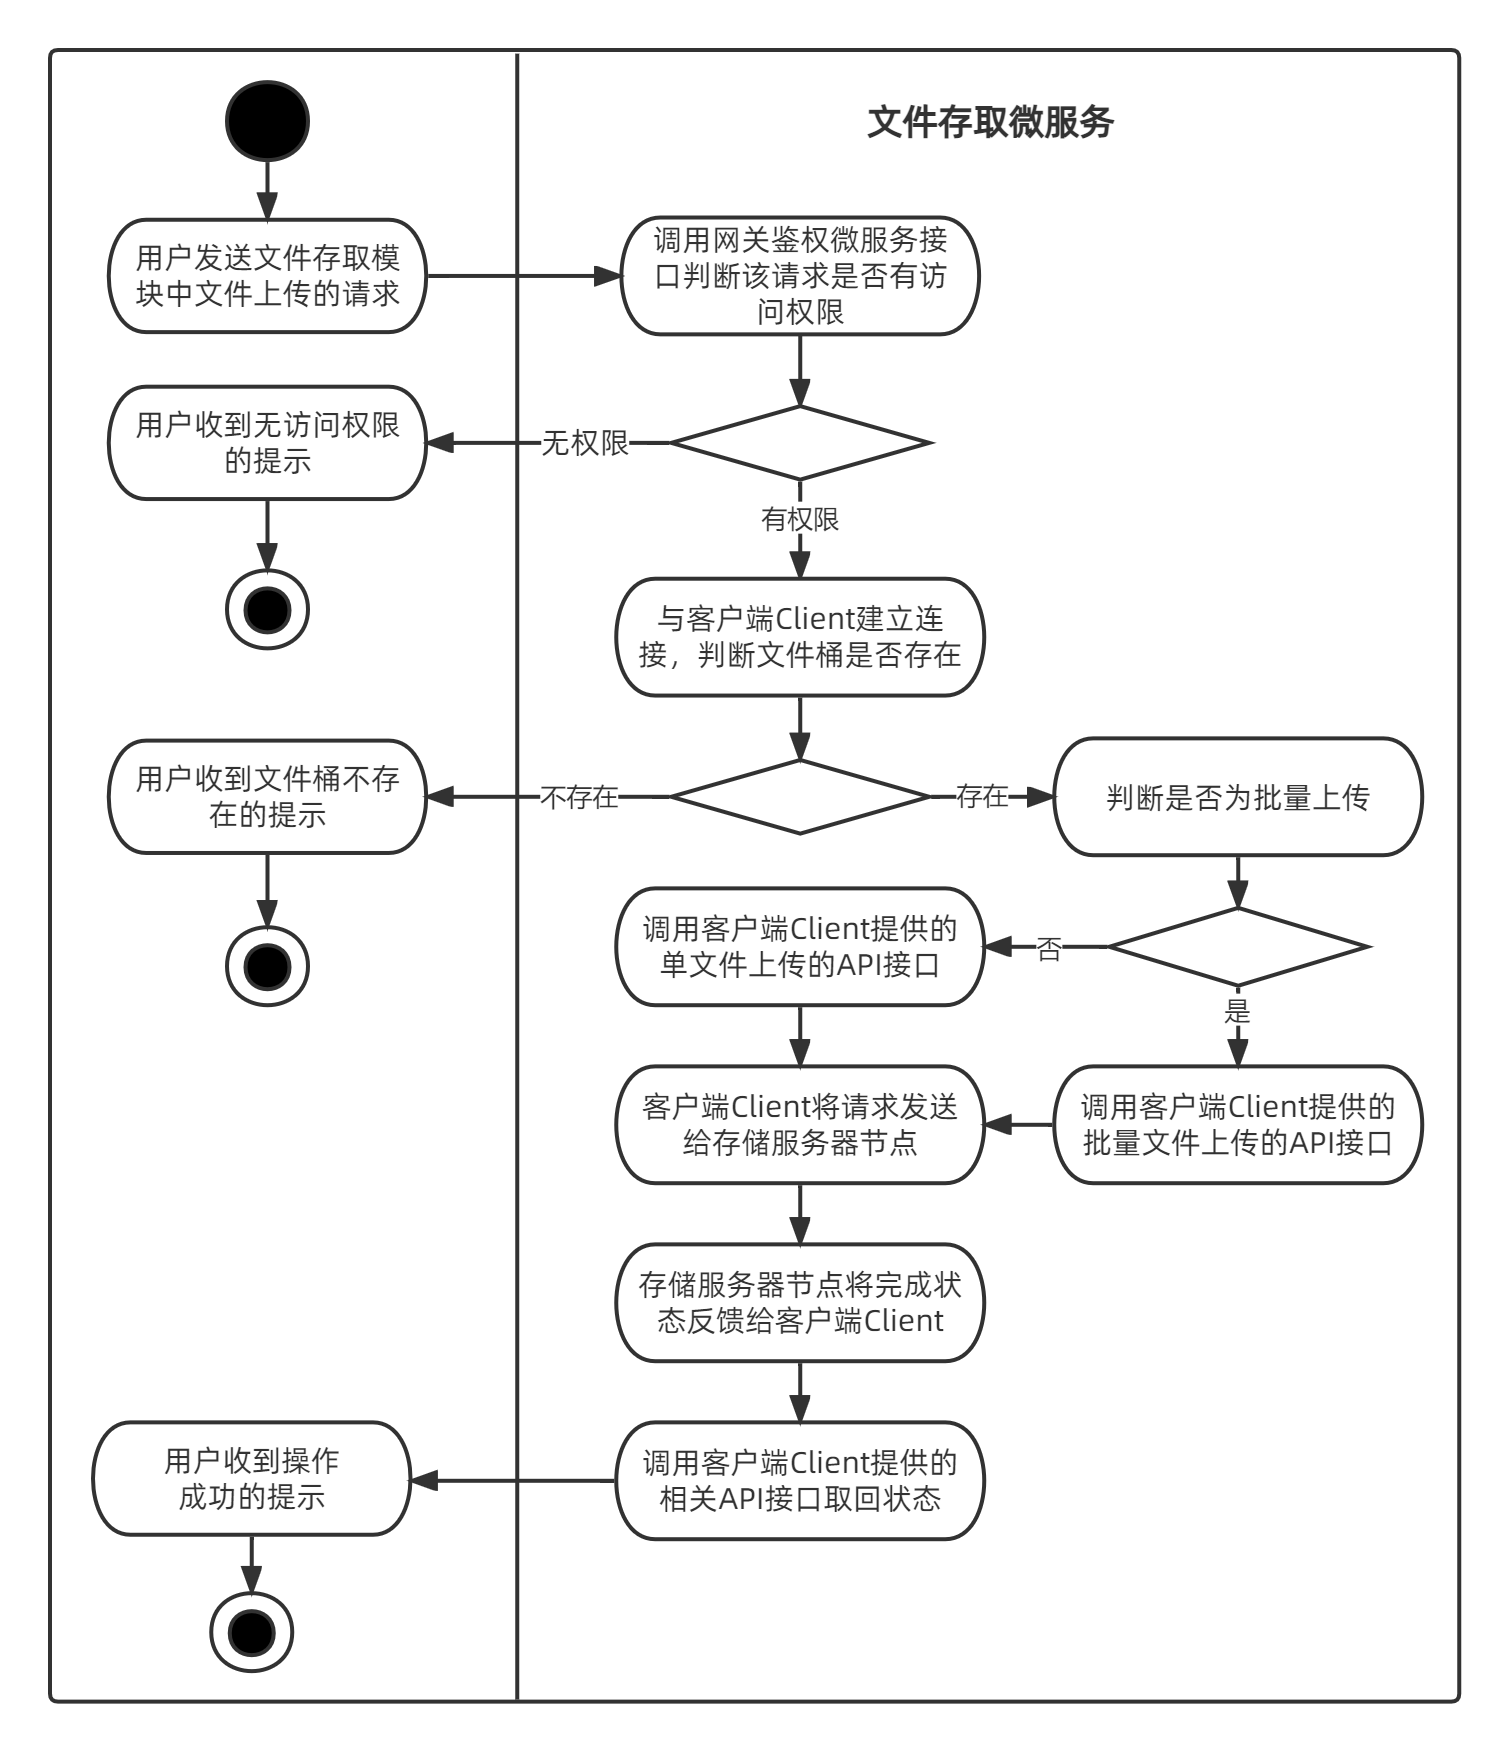
\includegraphics[width=0.8\textwidth]{my_figures/chapter4/文件上传活动图.png}
    \caption{文件上传活动图}
    \label{fig:文件上传活动图}
%     \note{注:图注的内容不宜放到图题中。}
\end{figure}

(3) 文件下载


文件下载功能主要是把文档从数据的主机下载到客户本地。和文件上传一样,也支持多文件批量下载,在下载过程中前端可以看到文件下载的实时进度,如果遇到网络波动或
断线,前端会有相应的反馈通知,网络故障时,系统会暂停文件的下载。整体的操作流程和文件上传类似。

(4) 文件删除

文件删除模块主要负责对用户Bucket中的文件进行在线删除。这里对文件的移除动作其实就是直接把文件从数据存放服务器中移除,支持对多文件批量移除,但移除时是会提醒前端进行确定,因此移除动作是不可逆的
。文件删除操作活动图如图\ref{fig:文件删除活动图}所示。

% \begin{figure}[htb]
%     \centering
%     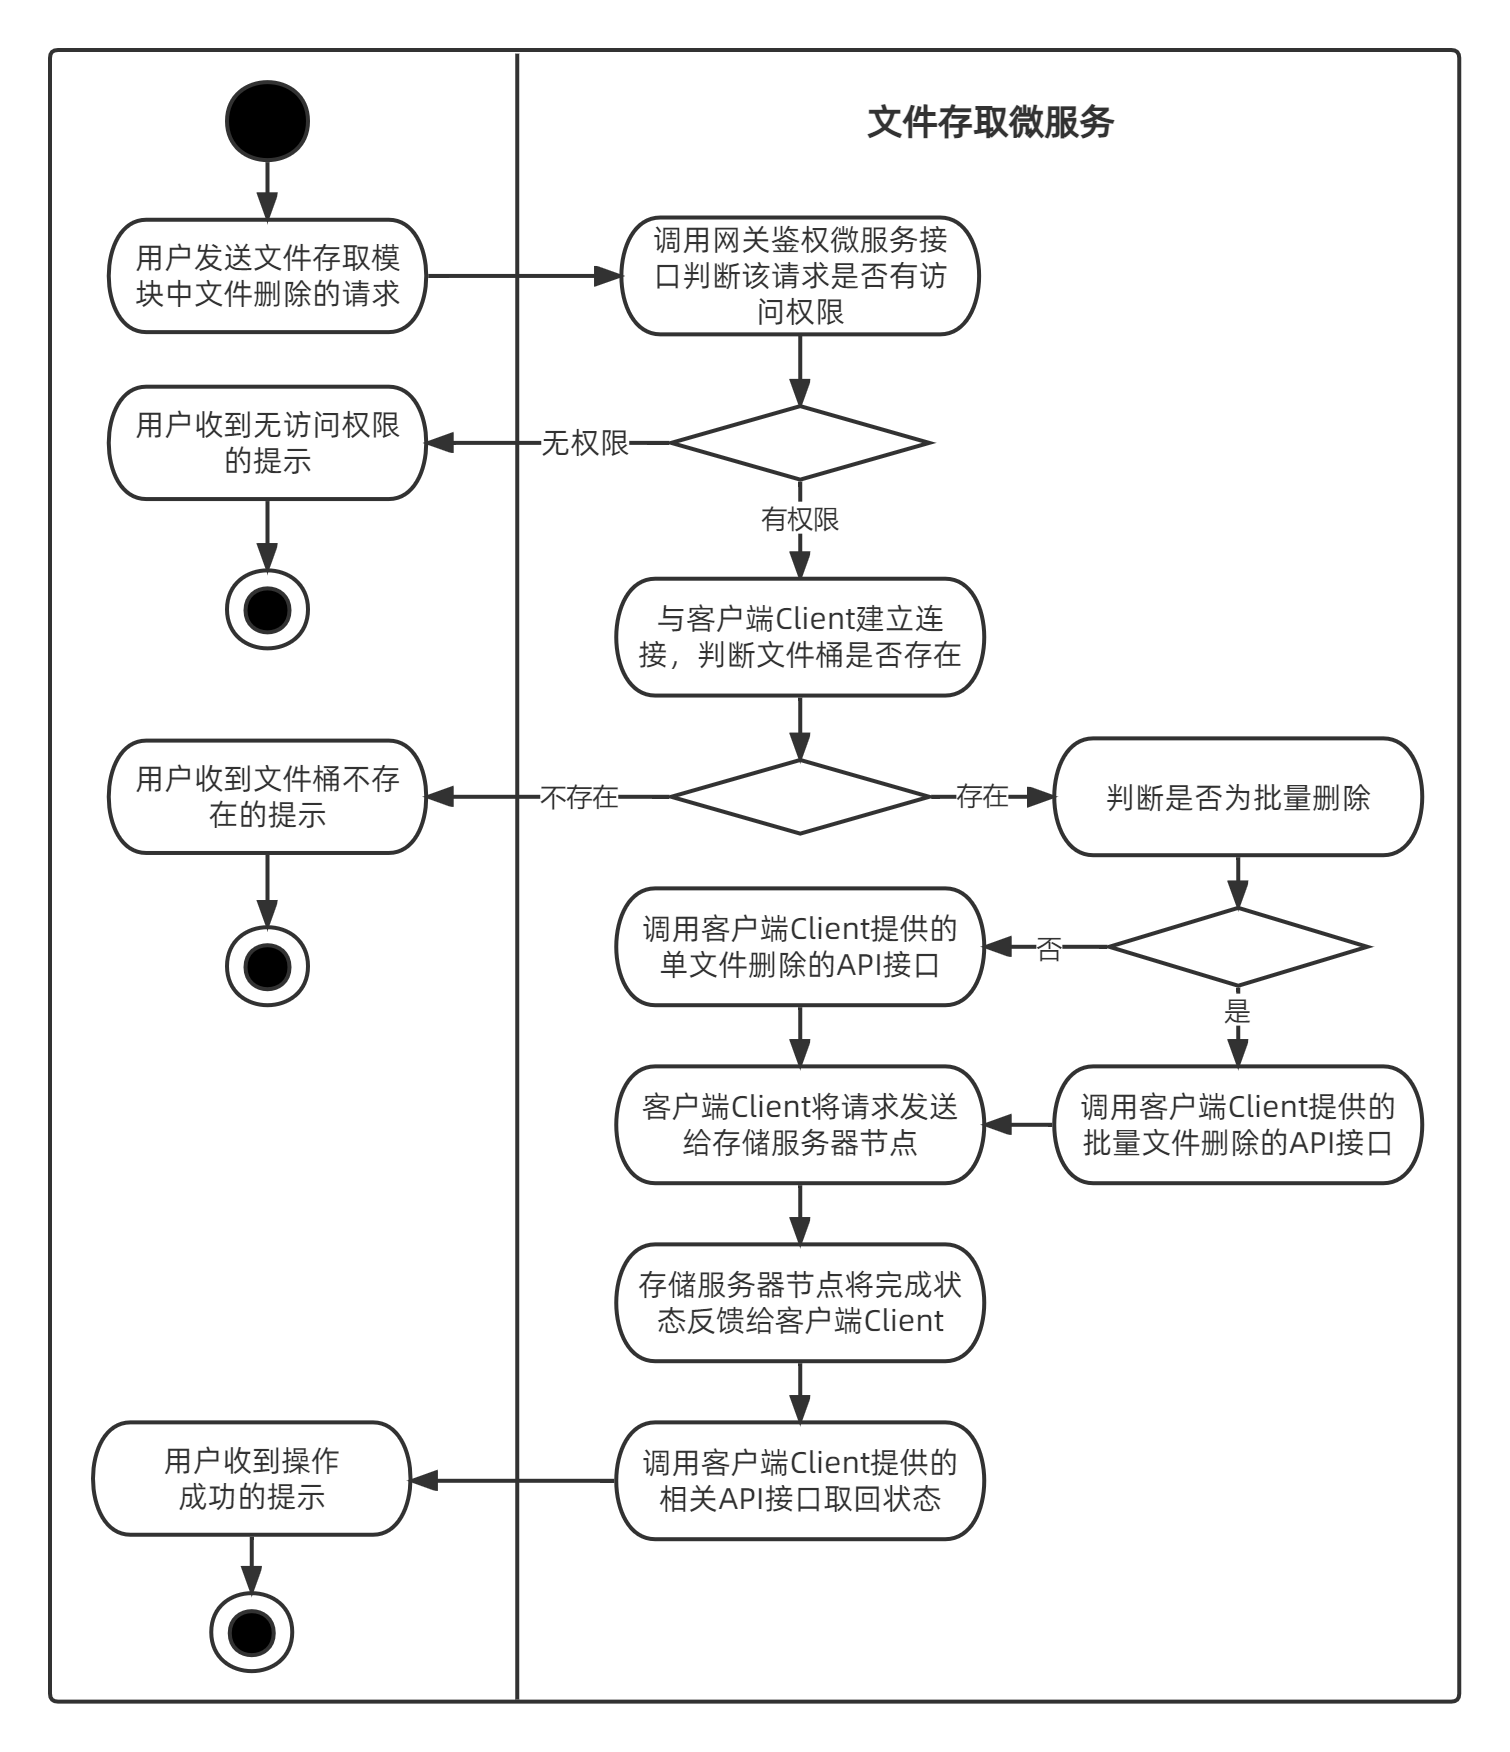
\includegraphics[width=0.8\textwidth]{my_figures/chapter4/文件删除活动图.png}
%     \caption{文件删除活动图}
%     \label{fig:文件删除活动图}
% %     \note{注:图注的内容不宜放到图题中。}
% \end{figure}

\subsection{系统维护模块}

系统维护模块主要是系统管理员用来对系统进行维护。系统维护模块主要包含三个子模块,分别是服务器管理子模块、集群管理子模块和日志管理子模块。只有管理员才有该模块的
访问权限。系统维护模块的功能结构图如图\ref{fig:系统维护模块功能结构图}所示。

\begin{figure}[htb]
    \centering
    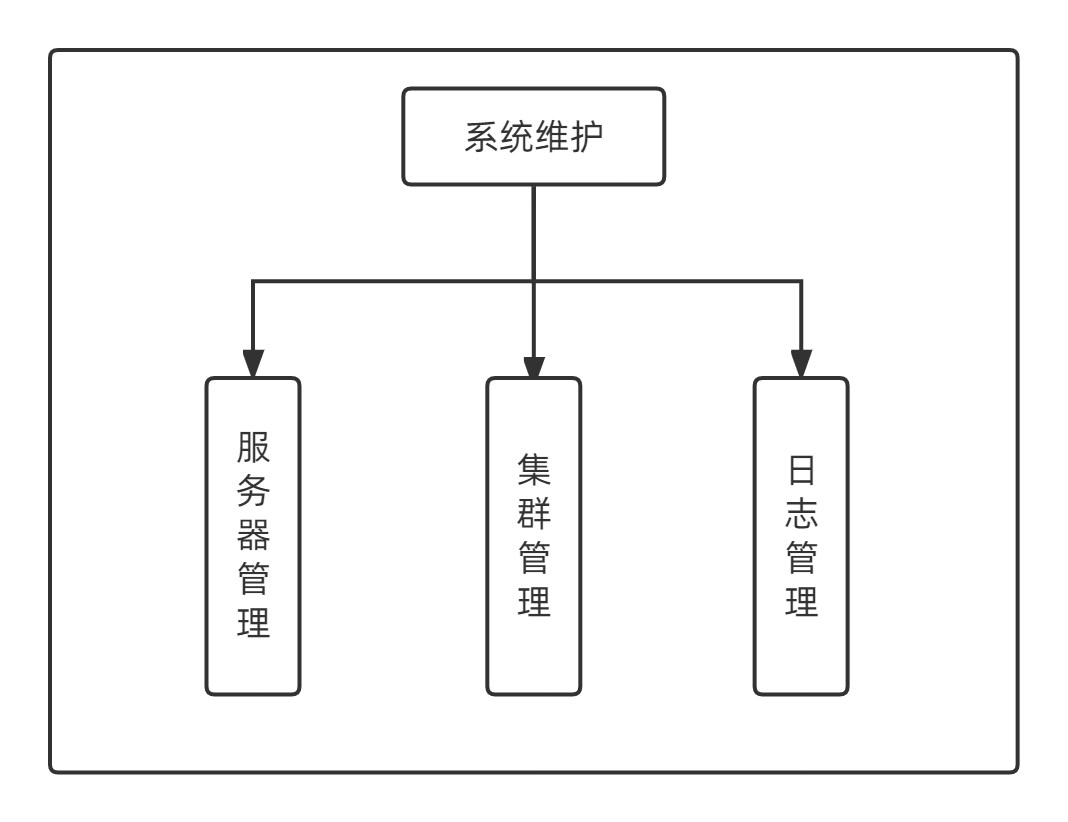
\includegraphics[width=0.8\textwidth]{my_figures/chapter4/系统维护模块功能结构图.png}
    \caption{系统维护模块功能结构图}
    \label{fig:系统维护模块功能结构图}
%     \note{注:图注的内容不宜放到图题中。}
\end{figure}

(1) 服务器管理

服务器管理模块主要负责对存储服务器进行启动和停止以及对服务器相关信息进行查看。该模块主要是方便运维人员对存储服务器进行维护,运维人员可以很方便在系统内对存储服务
进行停机、启动或重启的操作,也可以很直观的查看到存储服务器当前的信息,比如服务器版本、网络状况、已用容量、可用容量等信息。服务器管理活动图如图所示。

% \begin{figure}[htb]
%     \centering
%     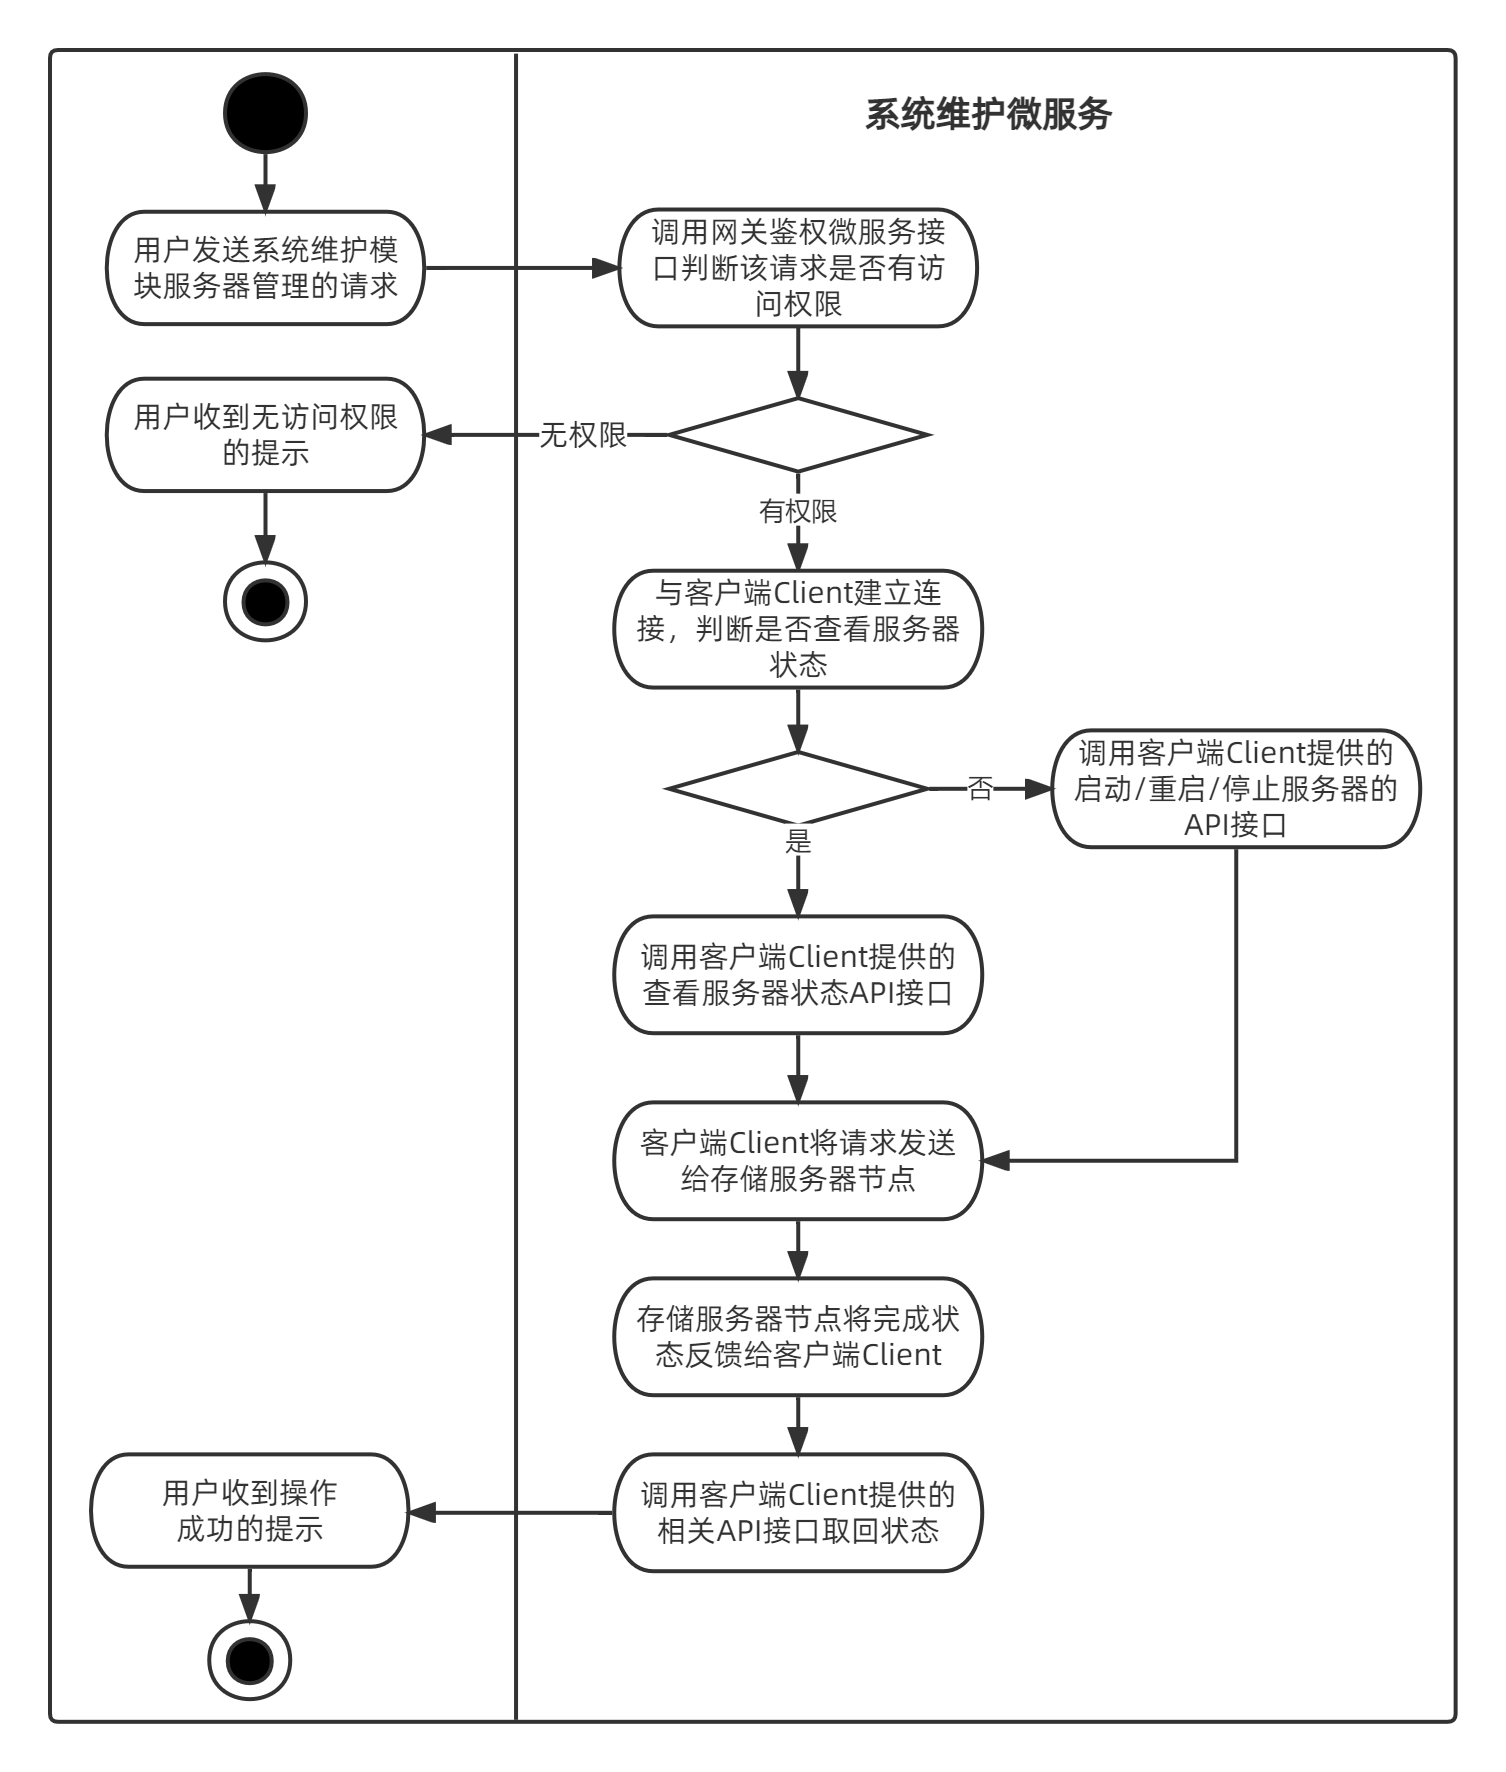
\includegraphics[width=0.8\textwidth]{my_figures/chapter4/服务器管理活动图.png}
%     \caption{服务器管理活动图}
%     \label{fig:服务器管理活动图}
% %     \note{注:图注的内容不宜放到图题中。}
% \end{figure}

(2) 集群管理

集群管理模块主要负责对服务器集群进行扩容、清理以及对集群状态进行查看。AliIO支持集群的直接扩容,在准备好准备扩充的另一个集群后,只需要在系统中输入集群的相关信息,
然后点击扩容即可,但是扩容之后需要重启当前扩容的集群才可生效。集群清理相当于将当前集群进行禁用,点击集群清理后同样需要重启集群方可生效。集群管理活动图如图所示。

% \begin{figure}[htb]
%     \centering
%     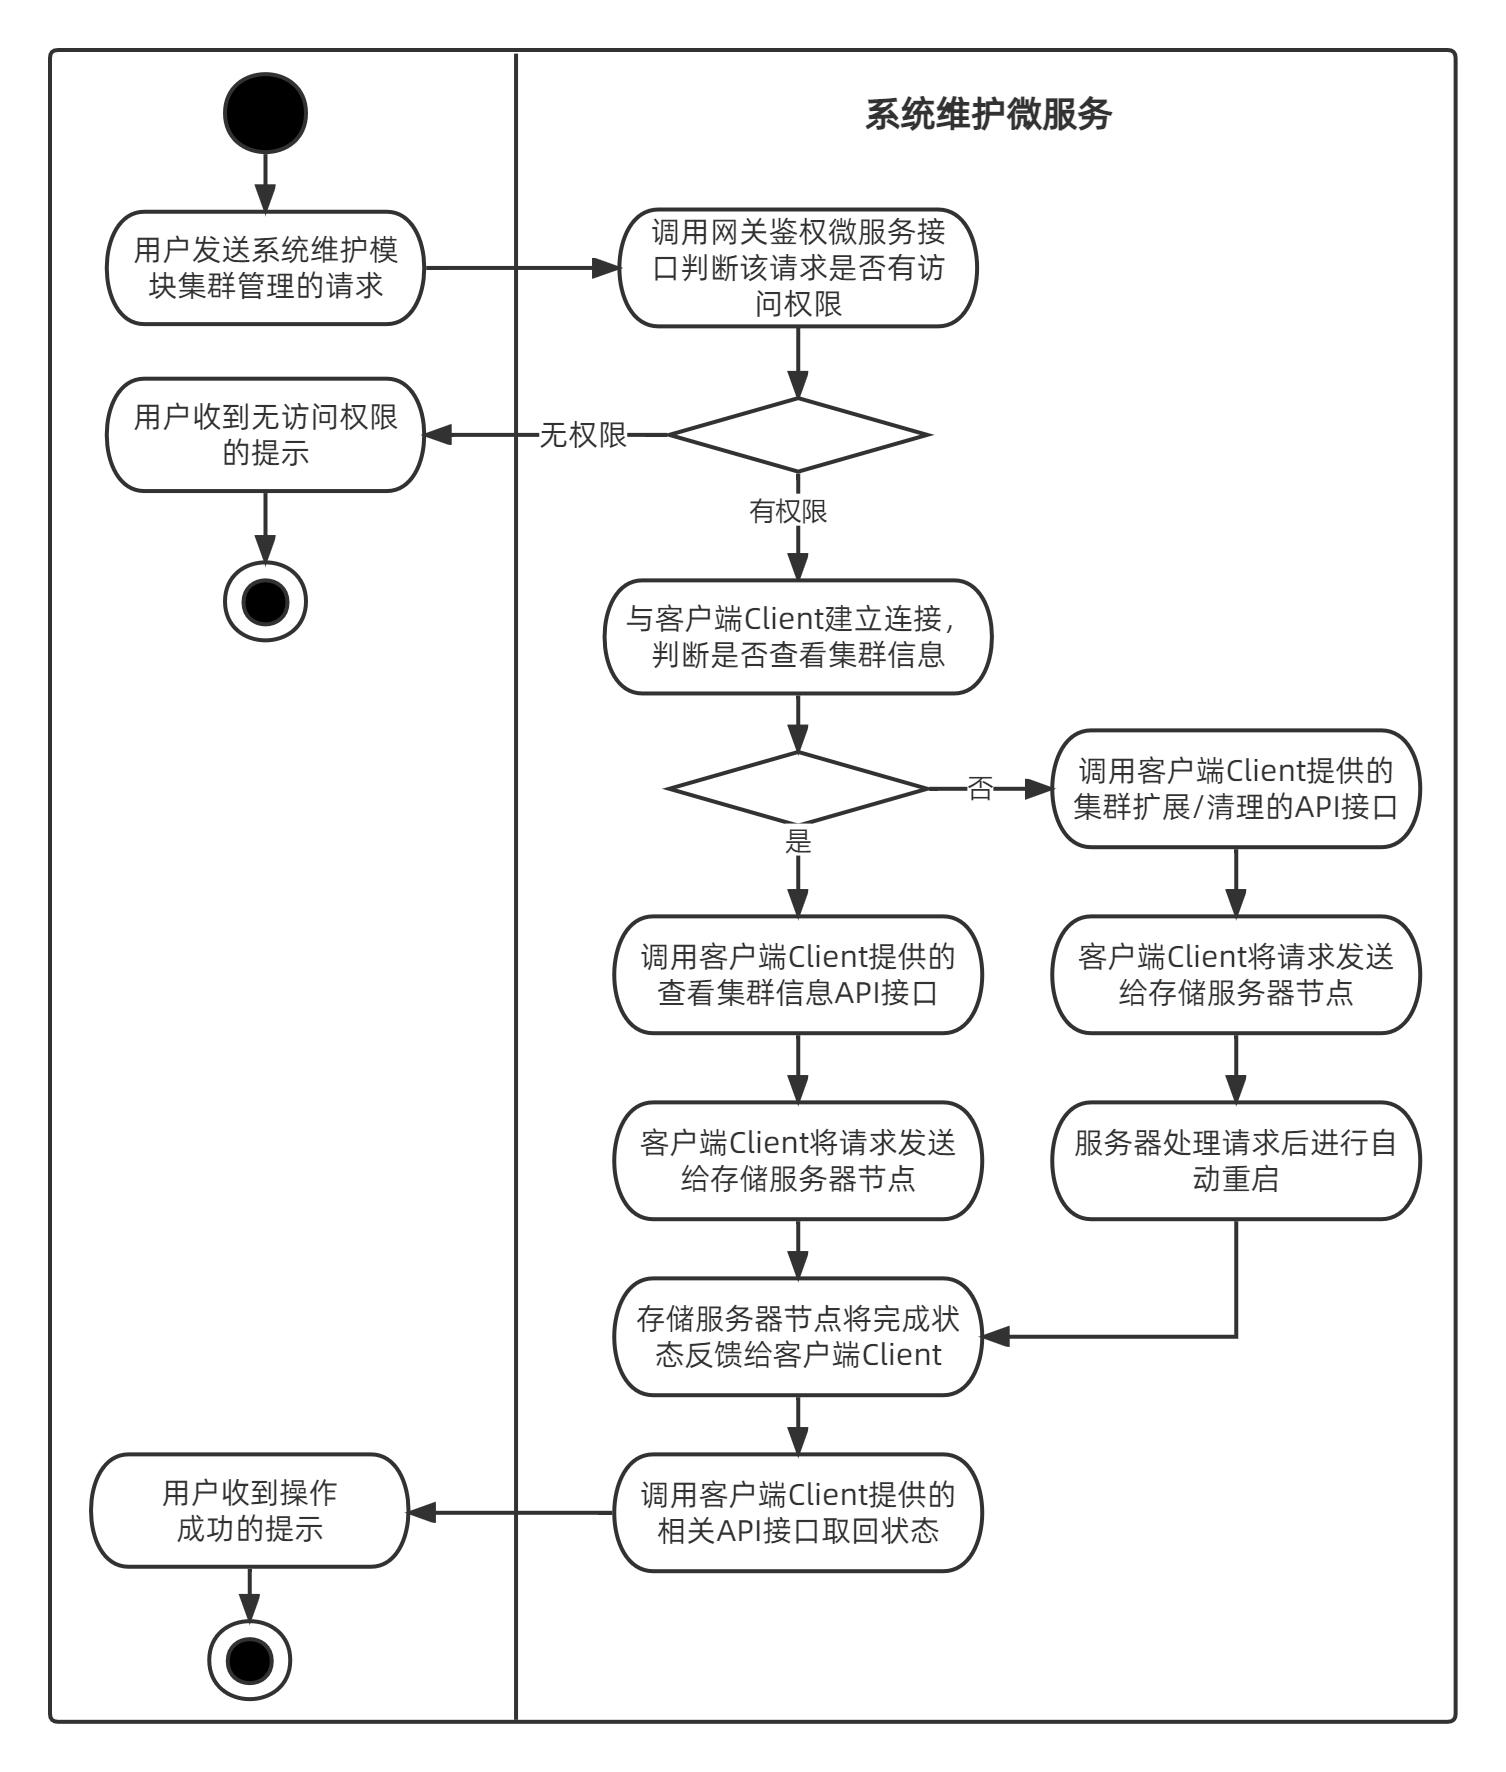
\includegraphics[width=0.8\textwidth]{my_figures/chapter4/集群管理活动图.png}
%     \caption{集群管理活动图}
%     \label{fig:集群管理活动图}
% %     \note{注:图注的内容不宜放到图题中。}
% \end{figure}

(3) 日志管理

日志管理模块主要负责对平台日志和存储日志进行管理。主要是对日志信息进行查看和删除操作。平台日志指的是用户登录管理平台后所进行的一些操作信息,存储日志是用户与存储
服务器进行交互后产生的一些操作信息,比如上传文件、删除文件等操作记录。平台日志主要是存储在MySQL数据库中,而存储日志位于存储服务器中。日志管理活动图如图所示。

% \begin{figure}[htb]
%     \centering
%     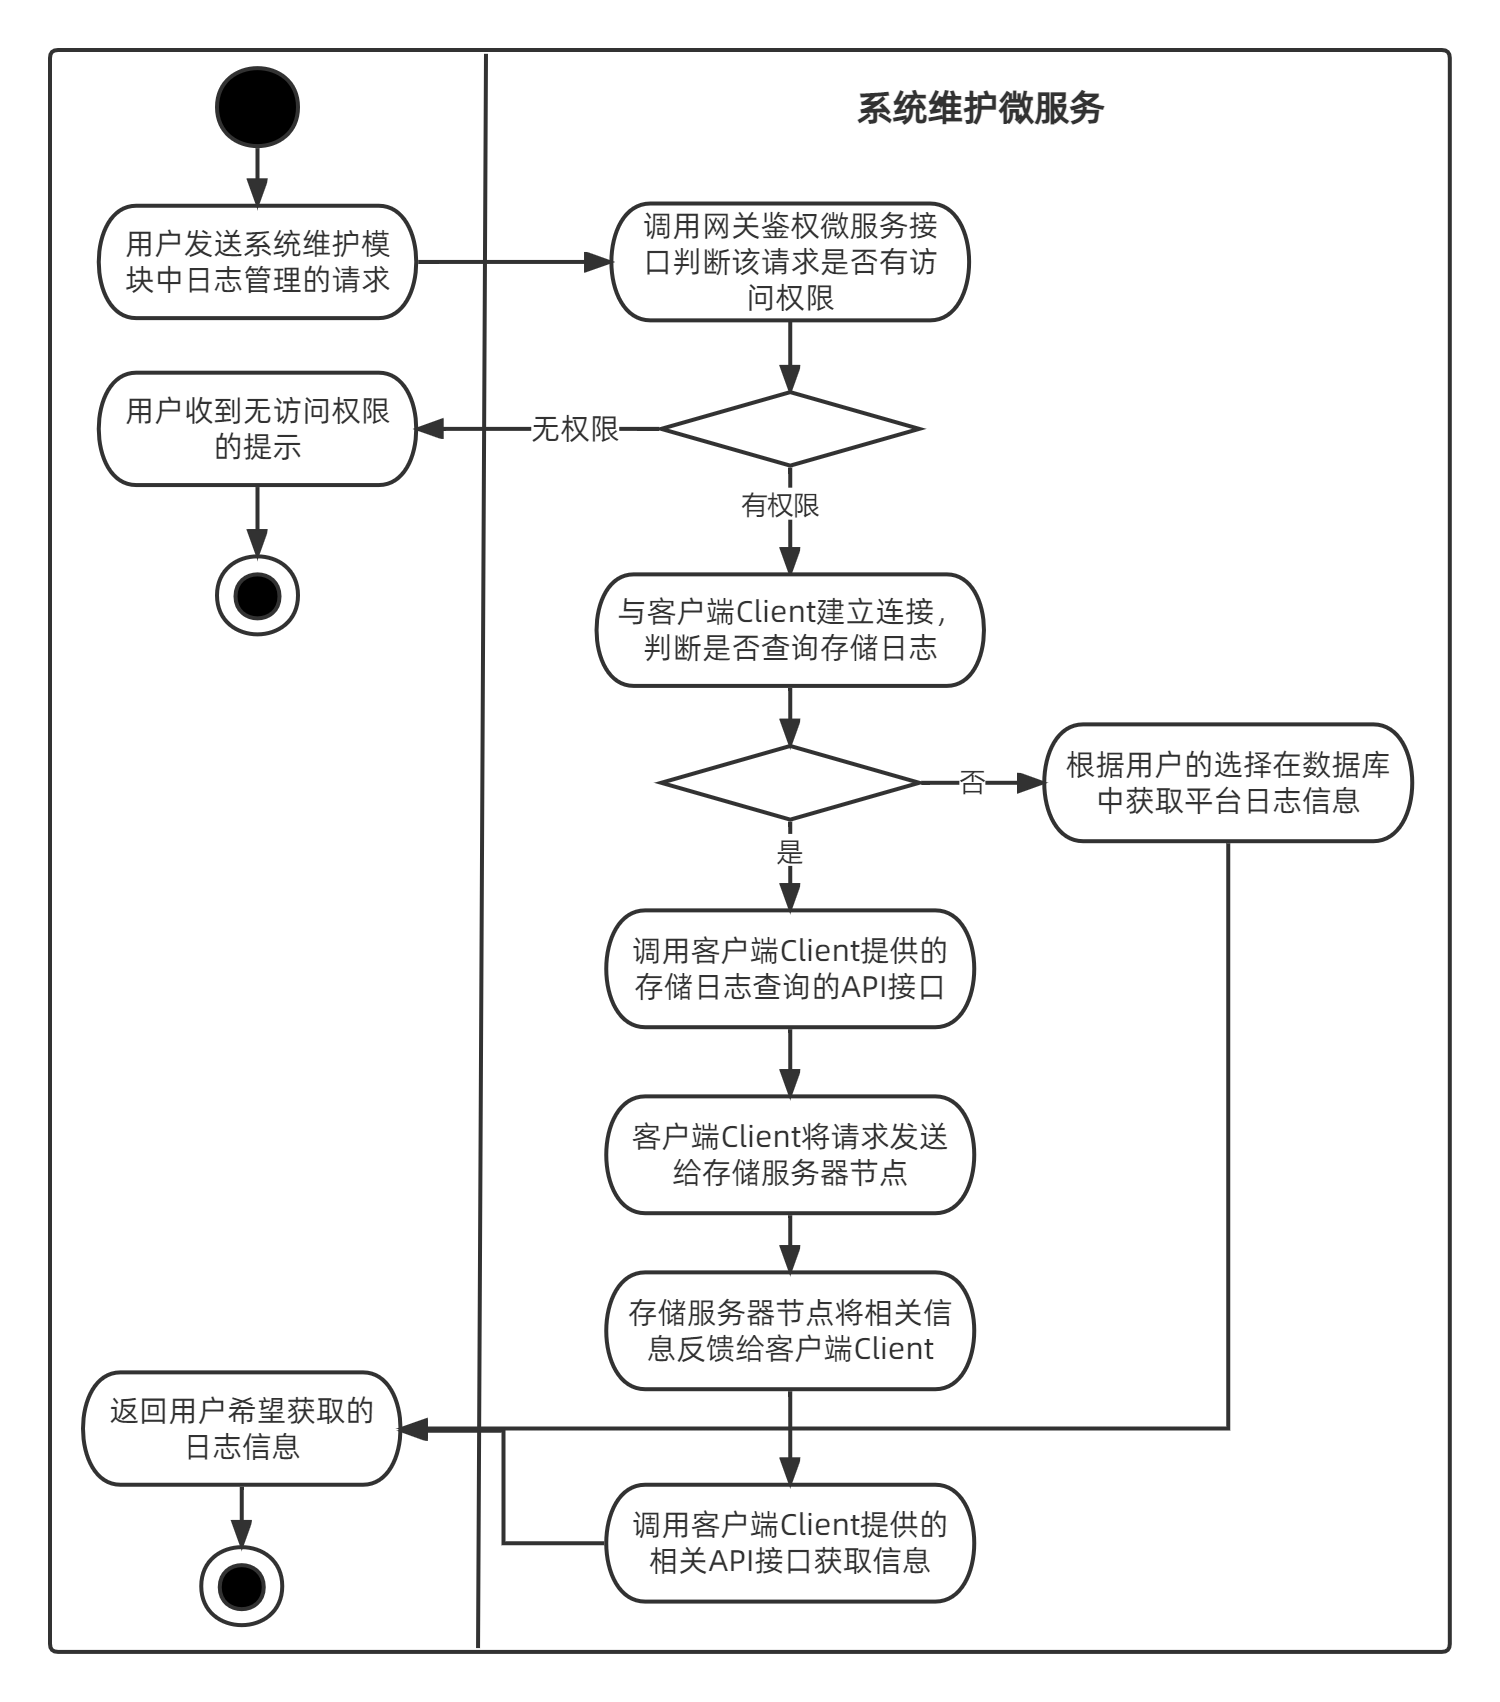
\includegraphics[width=0.8\textwidth]{my_figures/chapter4/日志管理活动图.png}
%     \caption{日志管理活动图}
%     \label{fig:日志管理活动图}
% %     \note{注:图注的内容不宜放到图题中。}
% \end{figure}

\section{数据库总体设计}

% 分布式对象存储管理系统的数据量十分庞大,随着使用用户的持续增长,大量的用户会使用该系统进行文件的上传和下载,这意味着越来越多的用户信息需要存储,所以良好的数据库设计
% 可以帮助处理大规模的数据,提高系统的整体运行效率。本系统后台数据库采用的是MySQL数据库,建立各部分数据库表。MySQL是一款具有高性能、强稳定性、支持高并发读写的关系
% 型数据库。因此,本系统MySQL 进行后台数据库的开发。

分布式个人文件存储与处理系统的信息量非常巨大,由于使用人群的持续增长,大批的个人都需要通过本信息系统完成个人文件的上传
与下发工作,这就意味着更大量的个人数据也需要存储,所以完善的信息库系统设置能够支持同时存储更大量的个人信息,从而大大提高
了信息库信息系统的总体工作效能。本管理平台信息应用的是MySQL资料库体系,包含了各部门信息库体系表。MySQL是一种具备高性
能、强安全性、支持多并发读写的关系式数据库。目前,日本利用MySQL进行了后台数据库系统的建设。

\subsection{数据库E-R图设计}

% 在系统数据库设计过程中,实体-关系图(E-R 图)有利于开发者更加清晰地理解系统数据之间的关系。根据第三章的系统需求分析, 可以看出系统的数据库实体有: 用户、 角色
% 、 权限、 存储服务器、日志信息。 实体之间的关系如图所示。



\subsection{数据库表概要设计}

% 本小节内容对 E-R 图中设计的实体进一步的描述, 确定实体所表示的数据表及数据表的功能, 下面是部分数据表的介绍。


(1) 用户信息表

用户信息列表中主要记载了使用账户的信息,如使用的账户、注册密码和电子邮箱等信息。

(2) 角色信息表

人物资料录都由人物ID,角色名称和人物密钥所构成。

(3) 权限信息表

授权信息列表主要记载着系统中的所有授权信息,而系统中的各个信息访问路径都对应着的授权。

(4) 用户角色关联表

客户端角色信息关系列表记载着玩家与人物的对应关系,每项信息由用户名称与人物代码构成。

(5) 权限角色关联表

授权人物信息关联列表记载了授权与人物的对应关联,每条记录由人物编号权限序号构成。

(6) 路由信息表

路由消URI、一组Predicate,以及一组Filter。

(7)服务器信息表

服务器信息表记录了存储服务器的基本信息,如服务器版本号、更新时间、对象数、桶数目、已用容量和可用容量等信息,这些信息可能会经常变化。

(8) 日志信息表

日志信息表记录了系统级别的日志信息,包括用户新增、删除、修改、登入登出,都会在日志表中留下相应的记录。

\section{本章小结}

% 本章从分布式对象存储管理系统的系统架构作为切入点,首先结合系统架构图对系统的逻辑架构和后端的技术架构进行了详细的分析,同时结合系统功能模块图对系统的功能模块
% 设计进行了阐述。之后根据各个模块的功能结构图和UML活动图,进一步对各个功能模块的设计进行了深入的介绍。最后借助E-R图对数据库表之间的关系进行了说明,并描述了相
% 关数据表所记录的内容。
本文以分布式对象数据处理技术的体系结构研究为重点,首先按照系统架构图对系统的逻辑构架以及后端的各种功能构成进行了细致的
描述,并按照系统的功能示意图对整个系统的功能模块构成进行了说明。然后通过各个单元的工作结构图以及UML活动流程图,又对各
个功能单元的工作做了深入的阐述。最后通过E-R图对数据库表间的关联做出了描述,并说明了各数据库表中信息的内容。